% Created 2019-09-16 Mon 12:00
% Intended LaTeX compiler: pdflatex
\documentclass[10pt,t]{beamer}
\usepackage[utf8]{inputenc}
\usepackage[T1]{fontenc}
\usepackage{graphicx}
\usepackage{grffile}
\usepackage{longtable}
\usepackage{wrapfig}
\usepackage{rotating}
\usepackage{amsmath}
\usepackage{textcomp}
\usepackage{amssymb}
\usepackage{capt-of}
\usepackage{hyperref}
\usetheme{default}
\author{L. Larrabee Strow}
\date{\today}
\title{\large All-Sky AIRS Anomaly Retrievals \newline
  using Zonally Gridded, Time Averaged \newline
  Brightness Temperature Spectra}
\subtitle{\footnotesize{AIRS Science Team Meeting}}
\date{\vspace{0.1in}\footnotesize{September 25, 2019 \vfill}}
\author{Sergio DeSouza--Machado\inst{1,2}, L. Larrabee Strow\inst{1,2}}
\institute[UMBC]{\inst{1} UMBC Physics Dept. \and \inst{2}UMBC JCET}
\input beamer_setup
\usetheme{metropolis}
\metroset{titleformat title=allcaps}
\renewcommand{\UrlFont}{\small\tt}
\renewcommand*{\UrlFont}{\footnotesize}
\tolerance=1000
\RequirePackage{fancyvrb}
\DefineVerbatimEnvironment{verbatim}{Verbatim}{fontsize=\footnotesize}
\begin{document}

\maketitle
\addtobeamertemplate{block begin}{
  \setlength{\parsep}{0pt}
  \setlength{\topsep}{3pt plus 2pt minus 2.5pt}
  \setlength{\itemsep}{0pt plus 0pt minus 2pt}
  \setlength{\partopsep}{2pt}
}

\section{Overview}
\begin{frame}
  \frametitle{Overview of talk}
  \begin{itemize}
  \item We are starting to produce long-term anomalies and trends directly from gridded (time and space)
        (radiance converted to Brightness Temperature BT)
  \item This process is very fast and easy to test in many ways.
  \item Details on our retrieved thermodynamic and cloud rates
  \end{itemize}
\end{frame}

% ---------------------------------------------------------------------
\section{Clear Sky vs ERA Anomalies}
\begin{frame}
  \frametitle{Clear Sky Retrievals}
  \begin{itemize}
    \item Larrabee's talk gives details (data from 2002/09 to 2018/08)
      \begin{itemize}
        \item 16 years of data divided into 16 day averages $\rightarrow$ 365 timesteps
        \item \textcolor{red}{AIRS observations sampled for CLEAR scenes in these bins}
        \item binned into 40 equal area latitude bins (thinner in equator/thicker at polar regions)
        \item BT anomalies and average ERA profiles for all 365 timesteps
      \end{itemize}
    \item kCARTA analytic jacobians for surface temperature, T(z), WV(z),O3(z)
    \item Ran off kCARTA at t=0 to t=T to make ``finite difference'' column trace gas jacobians
          (CO2,N2O,CH4,CFC11,CFC12)
    \item Using these jacobians, we retrieved T(t,z), WV(t,z), O3(t,z), CO2(t), N2O(t), CH4(t), 
          CFC11(t), CFC12(t), surftemp(t)
          at each of the 40 latbins $\times $ 365 timesteps
  \end{itemize}
\end{frame}

%%%%%%%%%%%%%%%%%%%%%%%%%

\begin{frame}{Tropical ERA Clear Sky Geophysical Anomalies}
%% see /home/sergio/MATLABCODE/oem_pkg_run_sergio_AuxJacs/MakeProfs/plot_anomalies.m
\vspace{-0.35in}

\begin{columns}
\begin{column}{0.45\columnwidth}
\begin{block}{\footnotesize T(z,t)}
\vspace{-0.1in}
\begin{center}
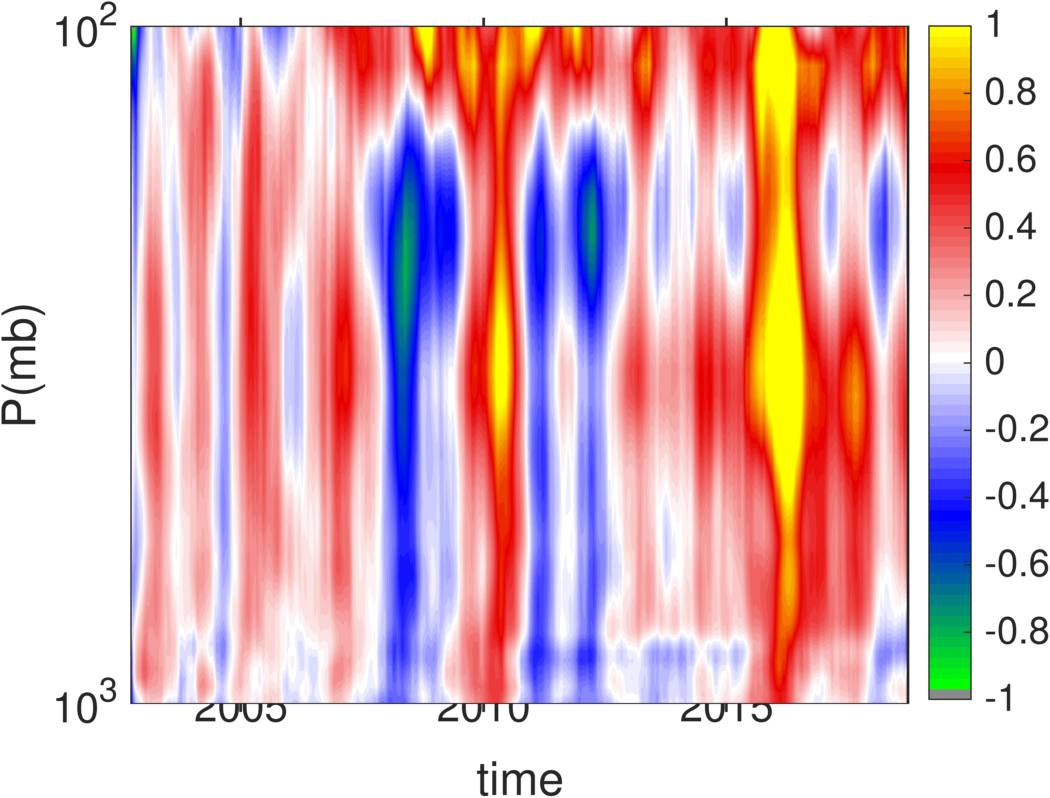
\includegraphics[width=\linewidth]{Figs/ClearAnom/era_clr_ptemp_anom_200209_201808.png}
\end{center}
\end{block}
\end{column}

\begin{column}{0.45\columnwidth}
\begin{block}{\footnotesize $frac$ WV(z,t)}
\vspace{-0.1in}
\begin{center}
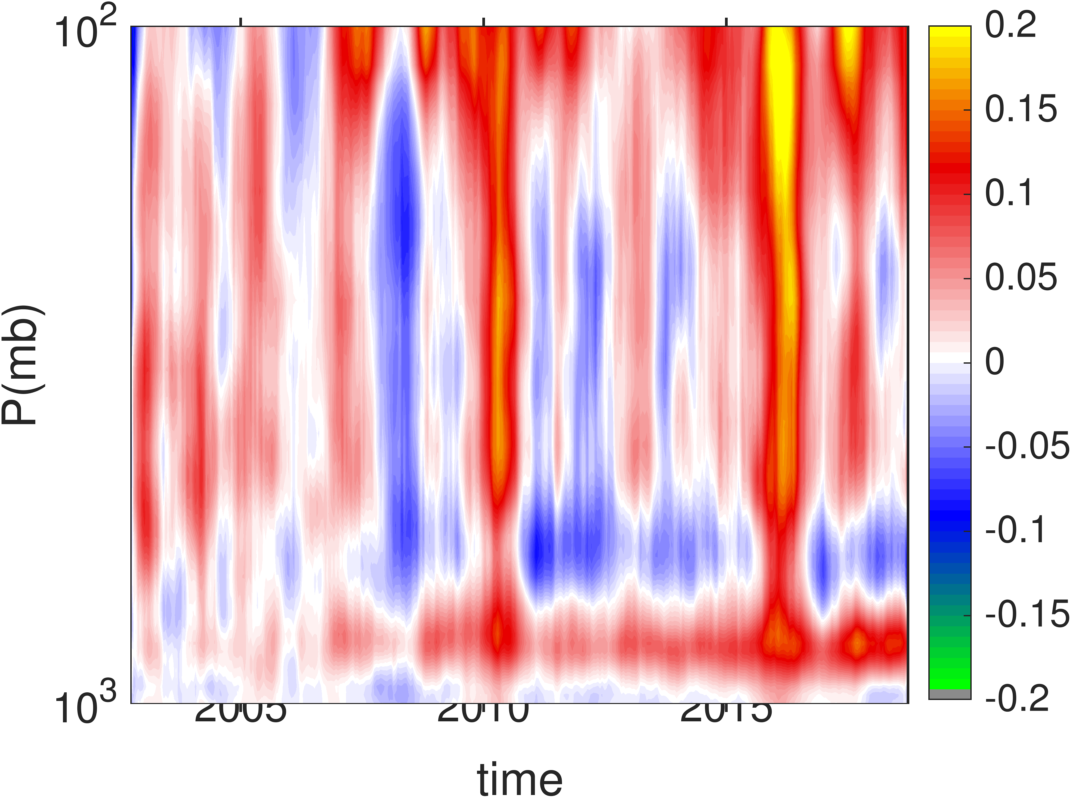
\includegraphics[width=\linewidth]{Figs/ClearAnom/era_clr_wv_anom_200209_201808.png}
\end{center}
\end{block}
\end{column}
\end{columns}

\vspace{-0.25in}

\begin{columns}
\begin{column}{0.45\columnwidth}
\begin{block}{\footnotesize $frac$ O3(z,t)}
\vspace{-0.1in}
\begin{center}
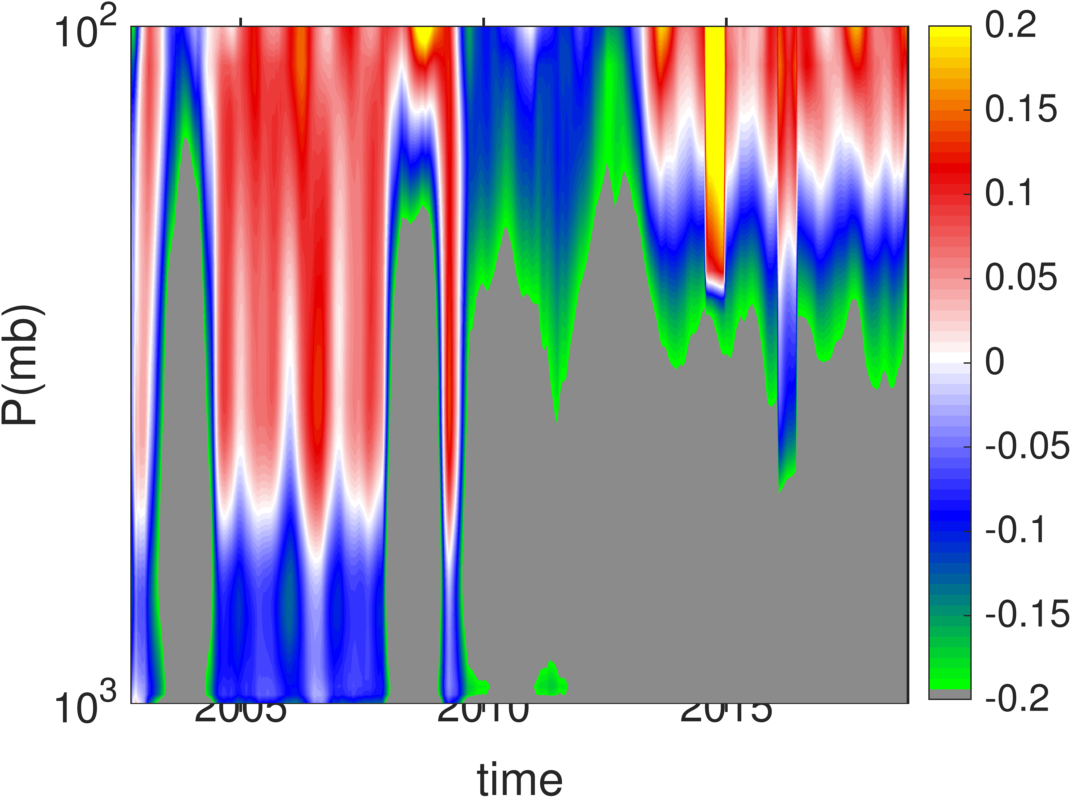
\includegraphics[width=\linewidth]{Figs/ClearAnom/era_clr_o3_anom_200209_201808.png}
\end{center}
\end{block}
\end{column}

\begin{column}{0.45\columnwidth}
%\begin{block}{\footnotesize Another Small Title}
%\vspace{-0.1in}
%\begin{center}
%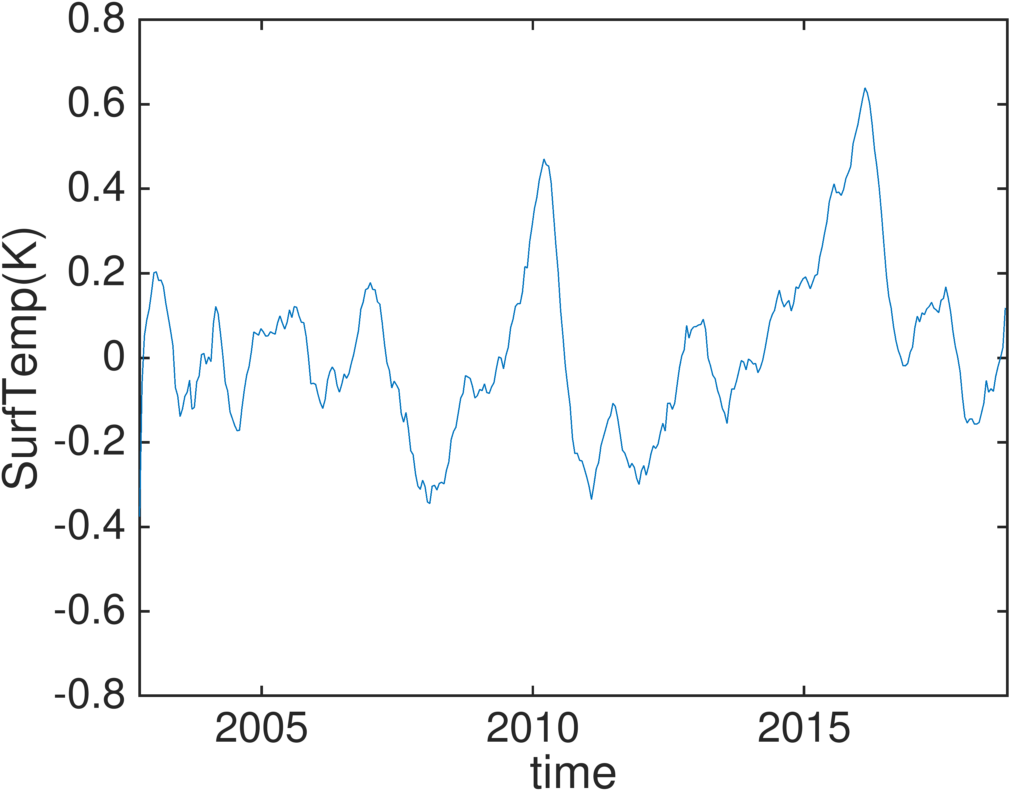
\includegraphics[width=\linewidth]{Figs/ClearAnom/era_clr_stemp_anom_200209_201808.png}
%\end{center}
%\end{block}

\end{column}
\end{columns}
\end{frame}

%%%%%%%%%%%%%%%%%%%%%%%%%

\begin{frame}{Tropical UMBC Retrieved Clear Sky CAL Geophysical Anomalies}
%% see /home/sergio/MATLABCODE/oem_pkg_run_sergio_AuxJacs/MakeProfs/plot_anomalies.m
\vspace{-0.35in}

\begin{columns}
\begin{column}{0.45\columnwidth}
\begin{block}{\footnotesize T(z,t)}
\vspace{-0.1in}
\begin{center}
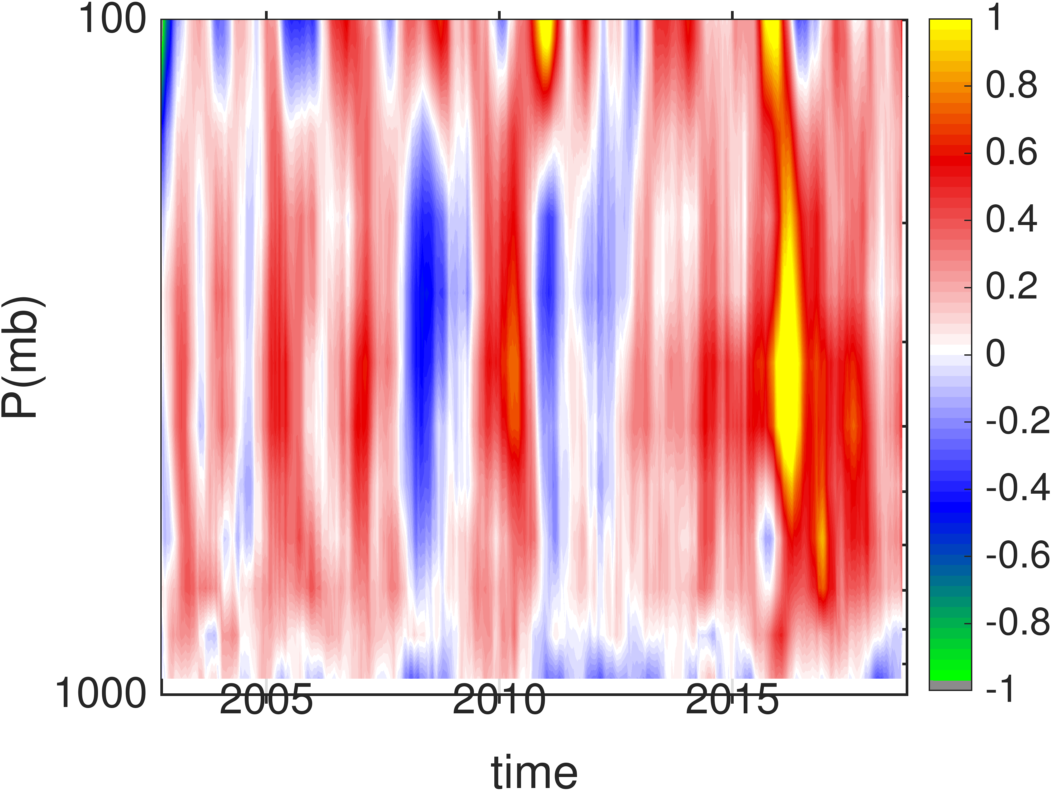
\includegraphics[width=\linewidth]{Figs/ClearAnom/umbc_clr_retr_cal_ptemp_anom_200209_201808.png}
\end{center}
\end{block}
\end{column}

\begin{column}{0.45\columnwidth}
\begin{block}{\footnotesize $frac$ WV(z,t)}
\vspace{-0.1in}
\begin{center}
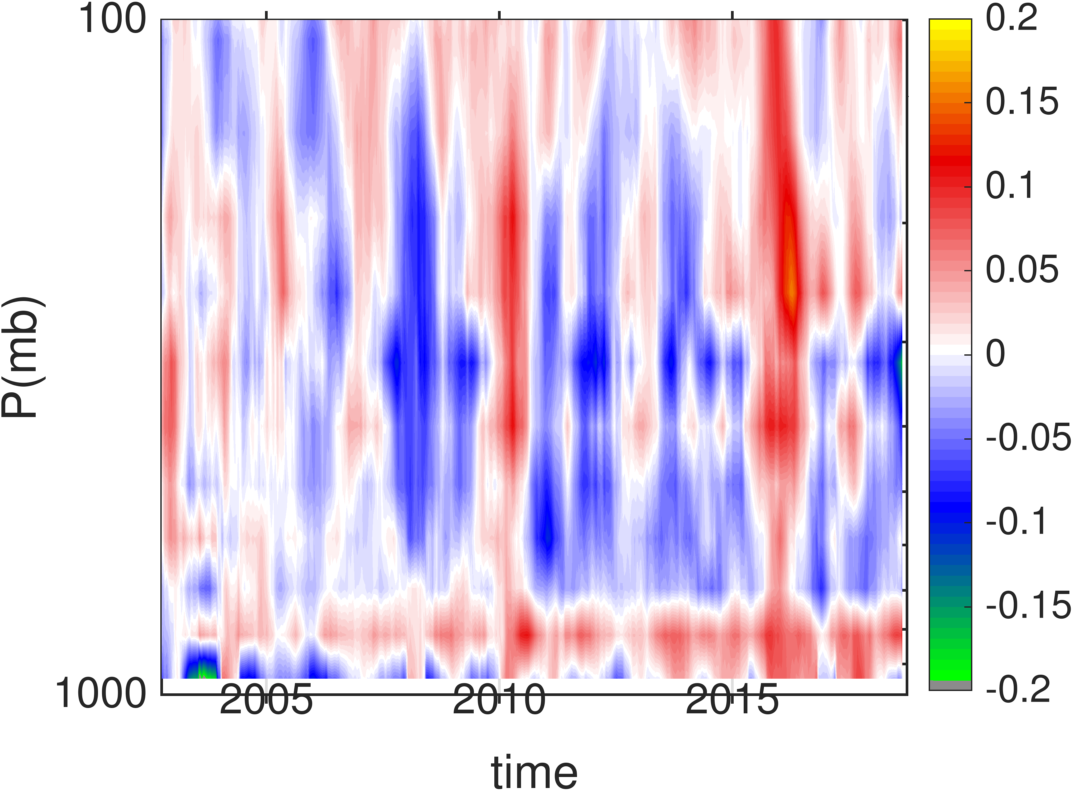
\includegraphics[width=\linewidth]{Figs/ClearAnom/umbc_clr_retr_cal_wv_anom_200209_201808.png}
\end{center}
\end{block}
\end{column}
\end{columns}

\vspace{-0.25in}

\begin{columns}
\begin{column}{0.45\columnwidth}
\begin{block}{\footnotesize $frac$ O3(z,t)}
\vspace{-0.1in}
\begin{center}
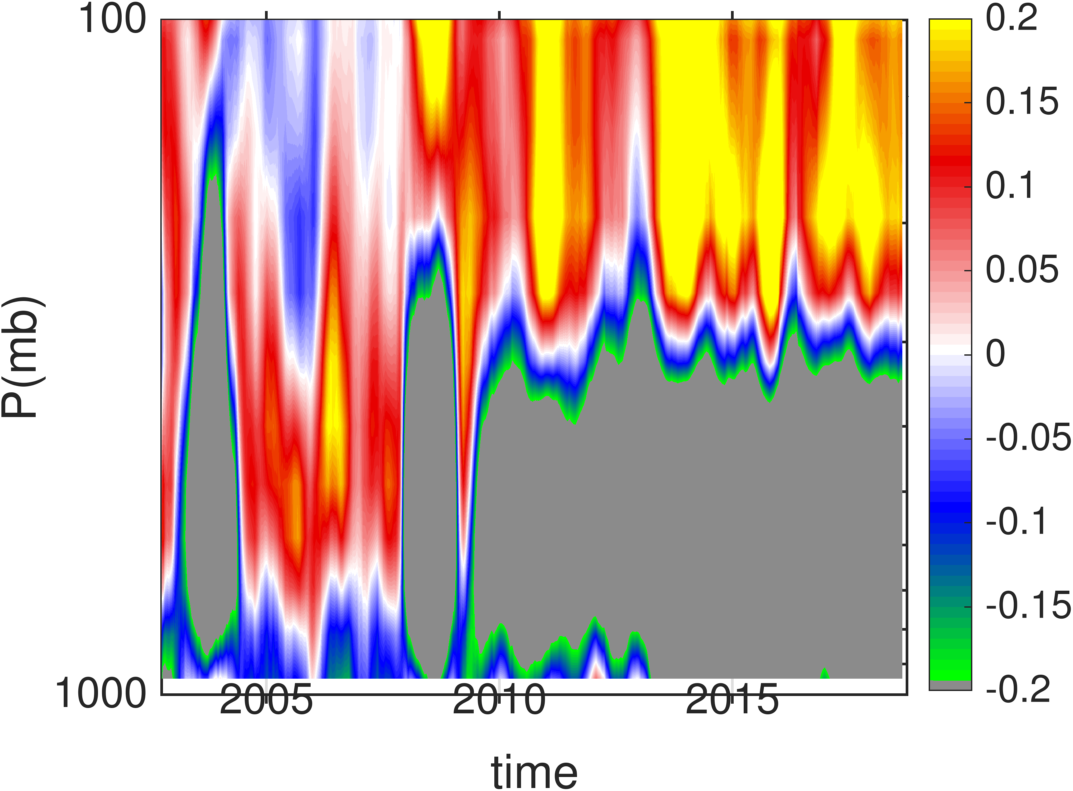
\includegraphics[width=\linewidth]{Figs/ClearAnom/umbc_clr_retr_cal_o3_anom_200209_201808.png}
\end{center}
\end{block}
\end{column}

\begin{column}{0.45\columnwidth}
%\begin{block}{\footnotesize Another Small Title}
%\vspace{-0.1in}
%\begin{center}
%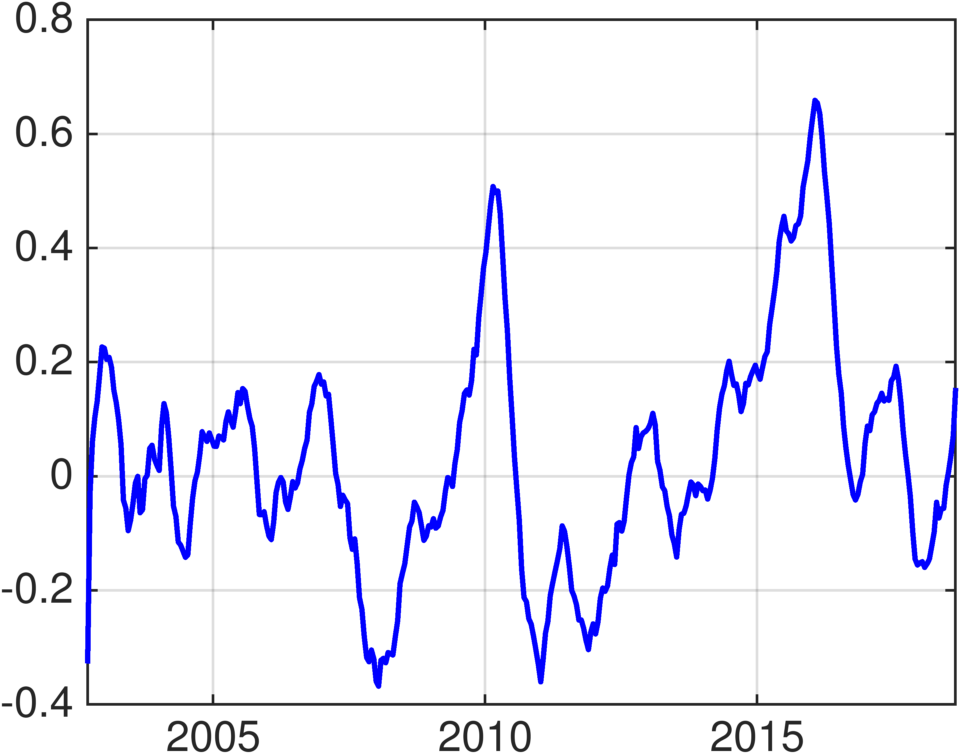
\includegraphics[width=\linewidth]{{Figs/ClearAnom/umbc_clr_retr_cal_stemp_anom_200209_201808.png}
%\end{center}
%\end{block}

\end{column}
\end{columns}
\end{frame}

%%%%%%%%%%%%%%%%%%%%%%%%%

\begin{frame}{Tropical UMBC Retrieved Clear Sky OBS Geophysical Anomalies}
%% see /home/sergio/MATLABCODE/oem_pkg_run_sergio_AuxJacs/MakeProfs/plot_anomalies.m
\vspace{-0.35in}

\begin{columns}
\begin{column}{0.45\columnwidth}
\begin{block}{\footnotesize T(z,t)}
\vspace{-0.1in}
\begin{center}
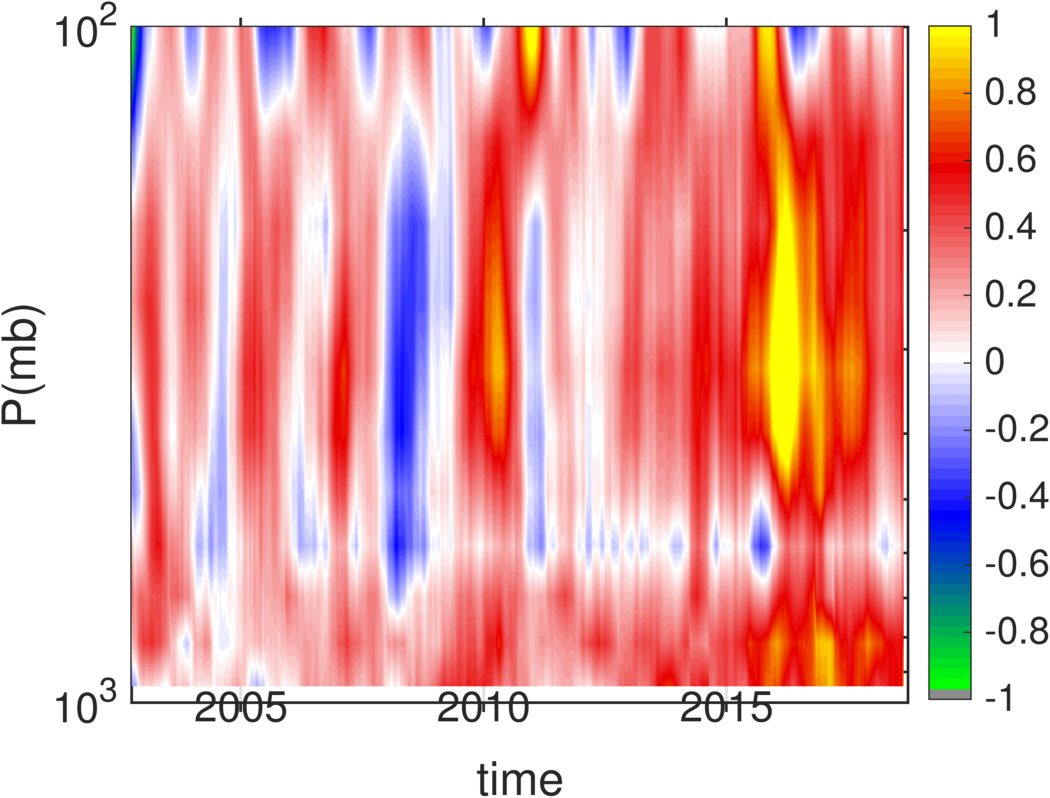
\includegraphics[width=\linewidth]{Figs/ClearAnom/umbc_clr_retr_obs_ptemp_anom_200209_201808.png}
\end{center}
\end{block}
\end{column}

\begin{column}{0.45\columnwidth}
\begin{block}{\footnotesize $frac$ WV(z,t)}
\vspace{-0.1in}
\begin{center}
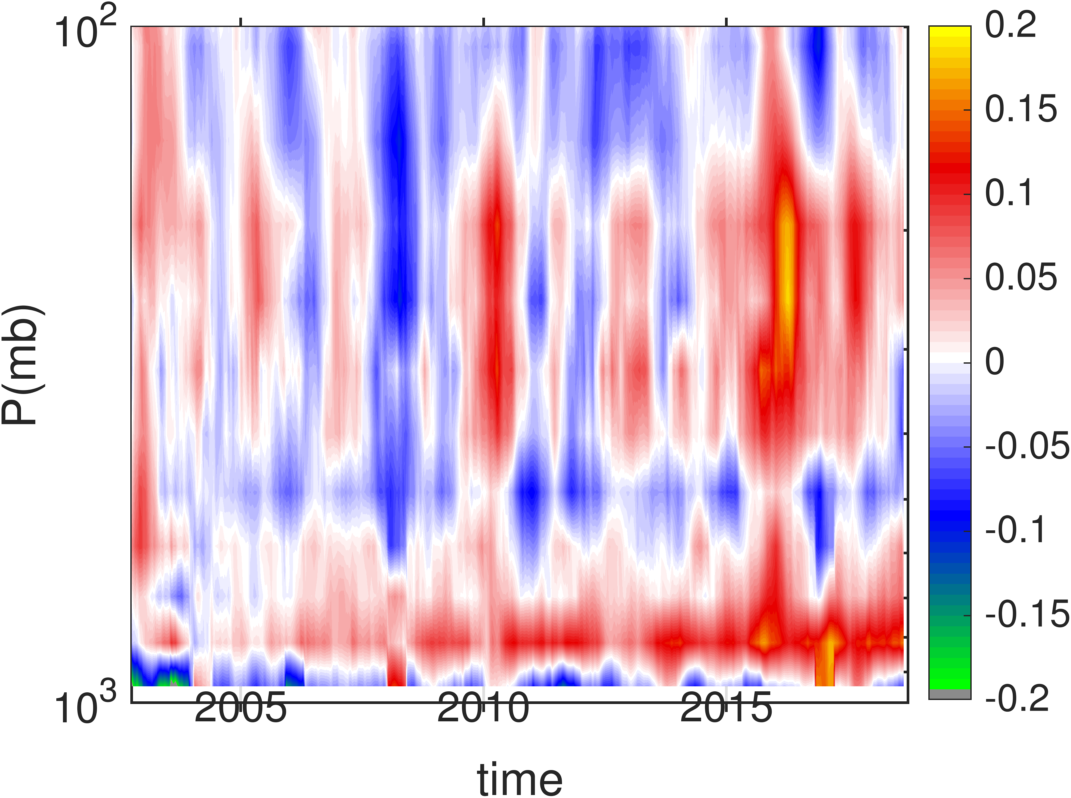
\includegraphics[width=\linewidth]{Figs/ClearAnom/umbc_clr_retr_obs_wv_anom_200209_201808.png}
\end{center}
\end{block}
\end{column}
\end{columns}

\vspace{-0.25in}

\begin{columns}
\begin{column}{0.45\columnwidth}
\begin{block}{\footnotesize $frac$ O3(z,t)}
\vspace{-0.1in}
\begin{center}
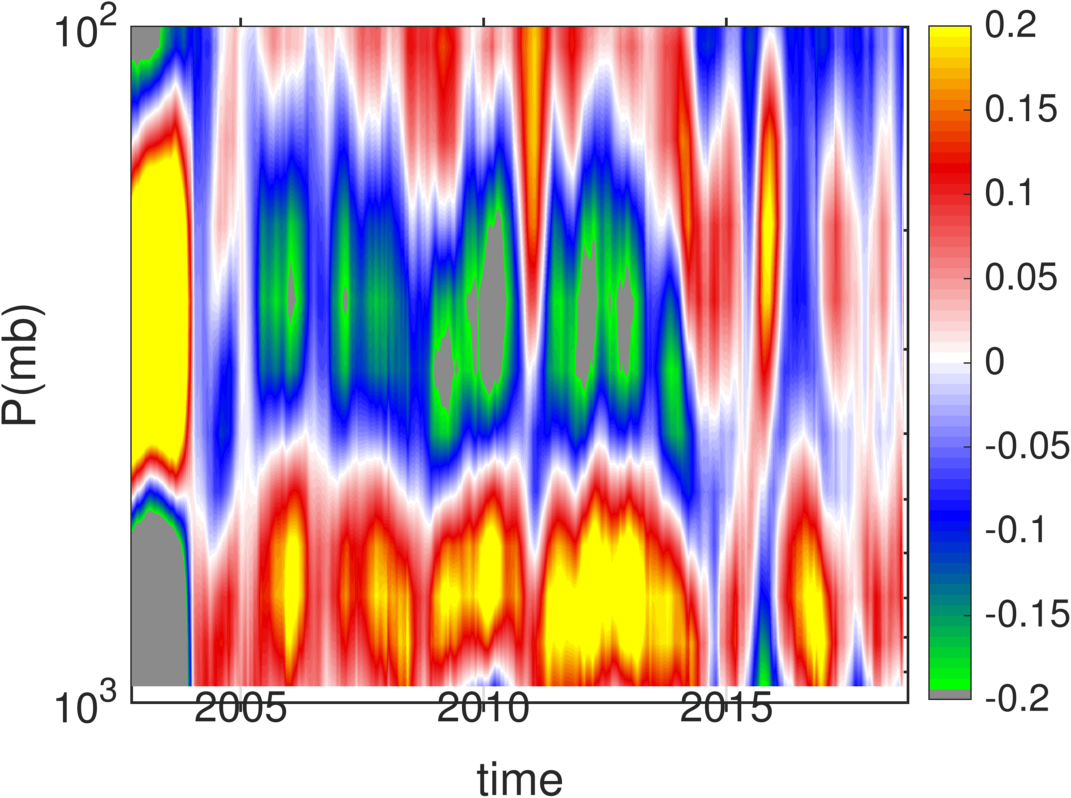
\includegraphics[width=\linewidth]{Figs/ClearAnom/umbc_clr_retr_obs_o3_anom_200209_201808.png}
\end{center}
\end{block}
\end{column}

\begin{column}{0.45\columnwidth}
%\begin{block}{\footnotesize Another Small Title}
%\vspace{-0.1in}
%\begin{center}
%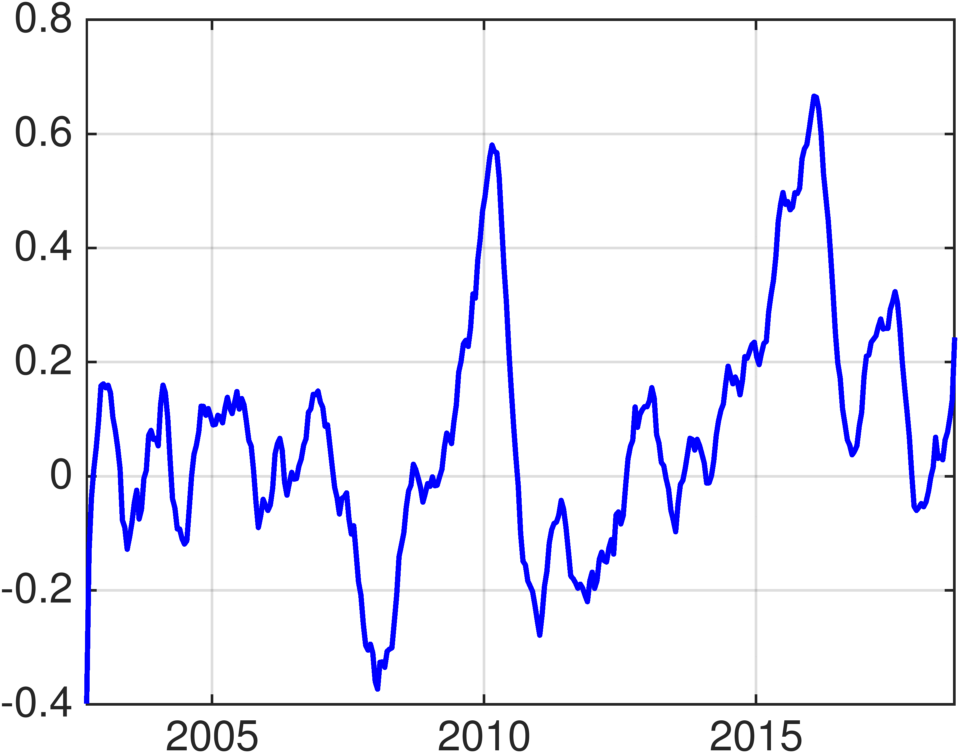
\includegraphics[width=\linewidth]{{Figs/ClearAnom/umbc_clr_retr_obs_stemp_anom_200209_201808.png}
%\end{center}
%\end{block}

\end{column}
\end{columns}
\end{frame}

%%%%%%%%%%%%%%%%%%%%%%%%%

\begin{frame}{UMBC Retrieved Clear Sky OBS Geophysical Anomalies $\rightarrow$ Geophysical Rates}
%% see /home/sergio/MATLABCODE/oem_pkg_run_sergio_AuxJacs/MakeProfs/plot_anomalies.m
\vspace{-0.35in}

\begin{columns}
\begin{column}{0.45\columnwidth}
\begin{block}{\footnotesize T(z,t)}
\vspace{-0.1in}
\begin{center}
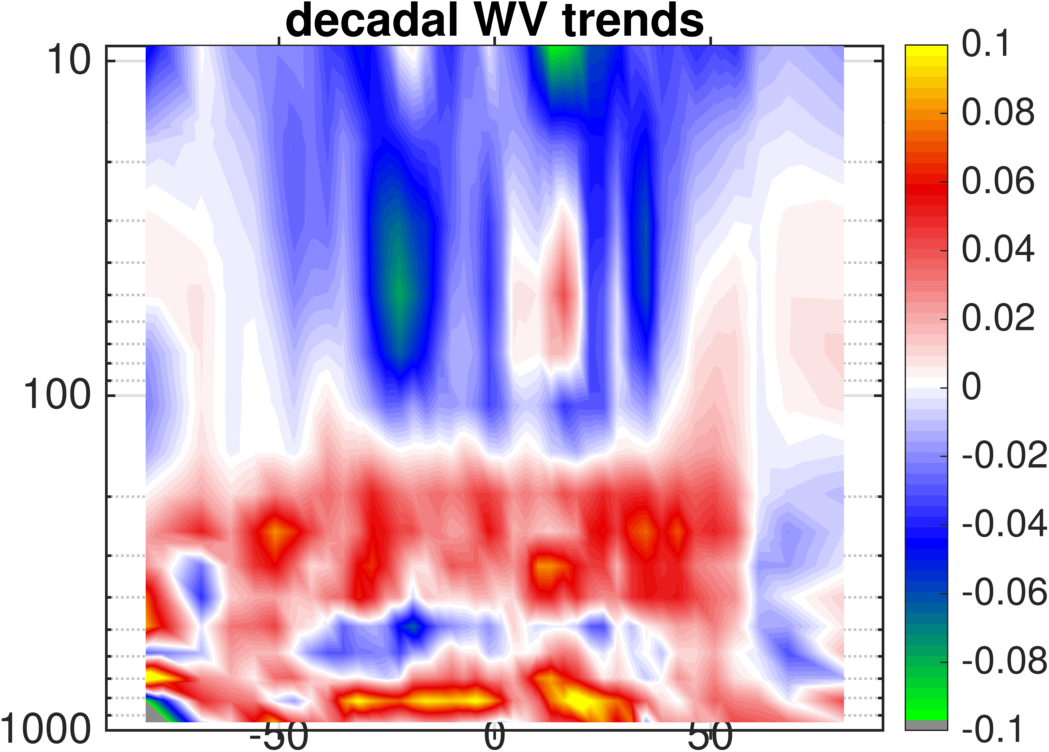
\includegraphics[width=\linewidth]{Figs/ClearAnom/umbc_clr_retr_obs_ptemp_rate_200209_201808.png}
\end{center}
\end{block}
\end{column}

\begin{column}{0.45\columnwidth}
\begin{block}{\footnotesize $frac$ WV(z,t)}
\vspace{-0.1in}
\begin{center}
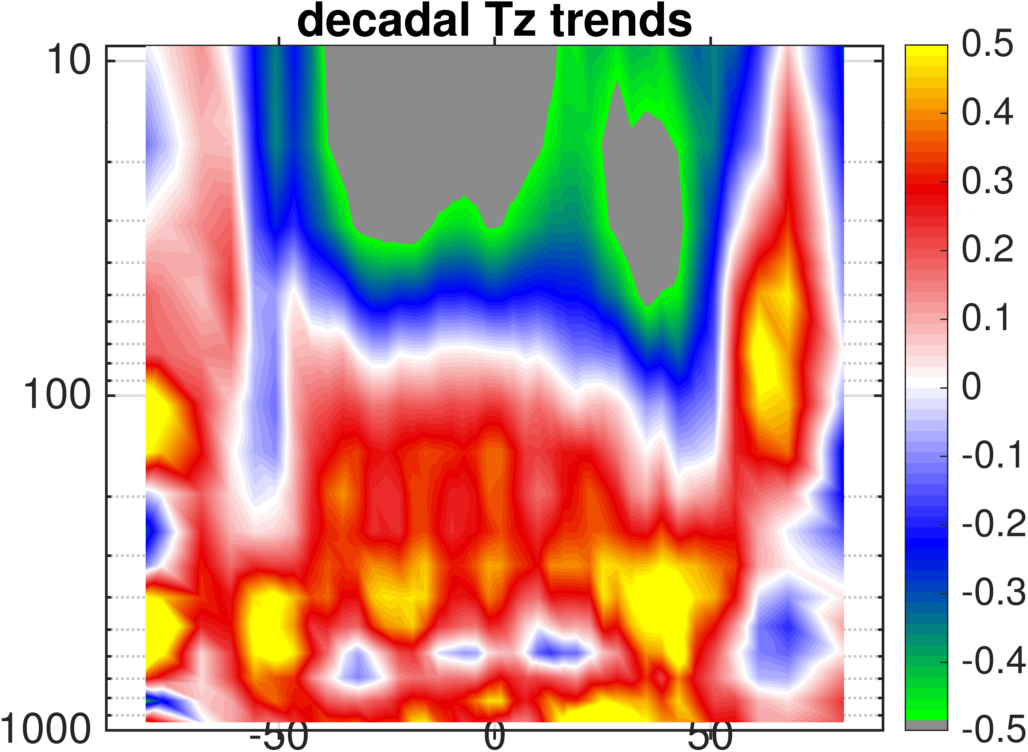
\includegraphics[width=\linewidth]{Figs/ClearAnom/umbc_clr_retr_obs_wv_rate_200209_201808.png}
\end{center}
\end{block}
\end{column}
\end{columns}

\vspace{-0.25in}

\begin{columns}
\begin{column}{0.45\columnwidth}
\begin{block}{\footnotesize $frac$ O3(z,t)}
\vspace{-0.1in}
\begin{center}
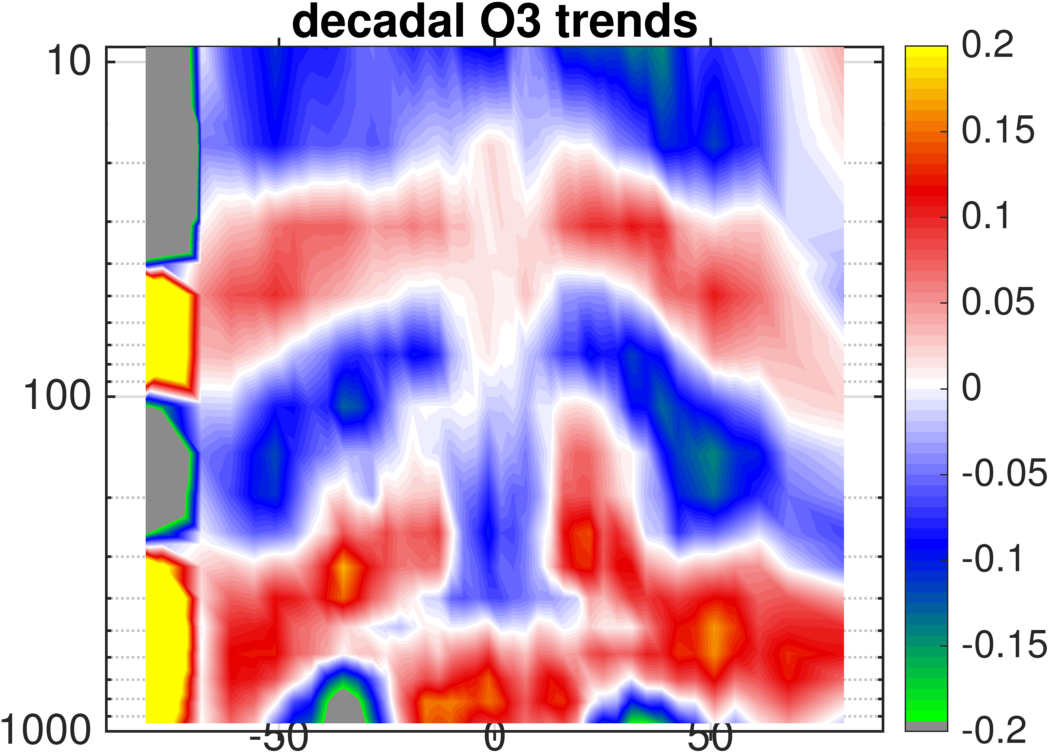
\includegraphics[width=\linewidth]{Figs/ClearAnom/umbc_clr_retr_obs_o3_rate_200209_201808.png}
\end{center}
\end{block}
\end{column}

\begin{column}{0.45\columnwidth}
%\begin{block}{\footnotesize Another Small Title}
%\vspace{-0.1in}
%\begin{center}
%\includegraphics[width=\linewidth]{{Figs/ClearAnom/umbc_clr_retr_obs_stemp_rate_200209_201808.png}
%\end{center}
%\end{block}

\end{column}
\end{columns}
\end{frame}

%%%%%%%%%%%%%%%%%%%%%%%%%

\begin{frame}{UMBC Retrieved Clear Sky CAL Geophysical Anomalies $\rightarrow$ Geophysical Rates}
%% see /home/sergio/MATLABCODE/oem_pkg_run_sergio_AuxJacs/MakeProfs/plot_anomalies.m
\vspace{-0.35in}

\begin{columns}
\begin{column}{0.45\columnwidth}
\begin{block}{\footnotesize T(z,t)}
\vspace{-0.1in}
\begin{center}
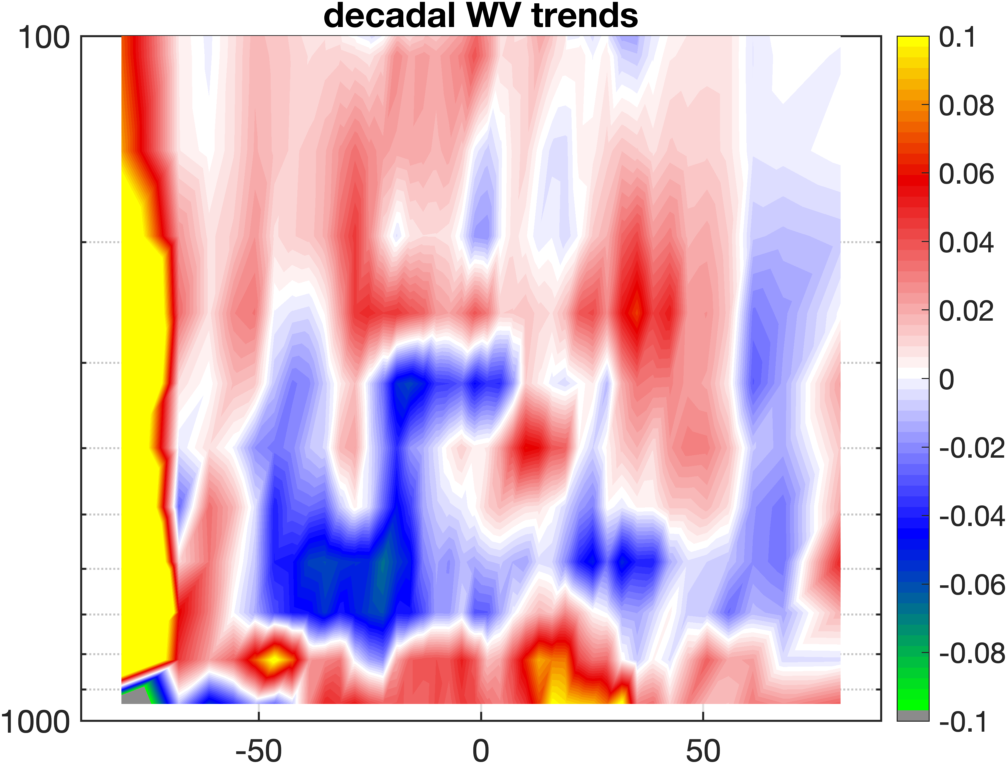
\includegraphics[width=\linewidth]{Figs/ClearAnom/umbc_clr_retr_cal_ptemp_rate_200209_201808.png}
\end{center}
\end{block}
\end{column}

\begin{column}{0.45\columnwidth}
\begin{block}{\footnotesize $frac$ WV(z,t)}
\vspace{-0.1in}
\begin{center}
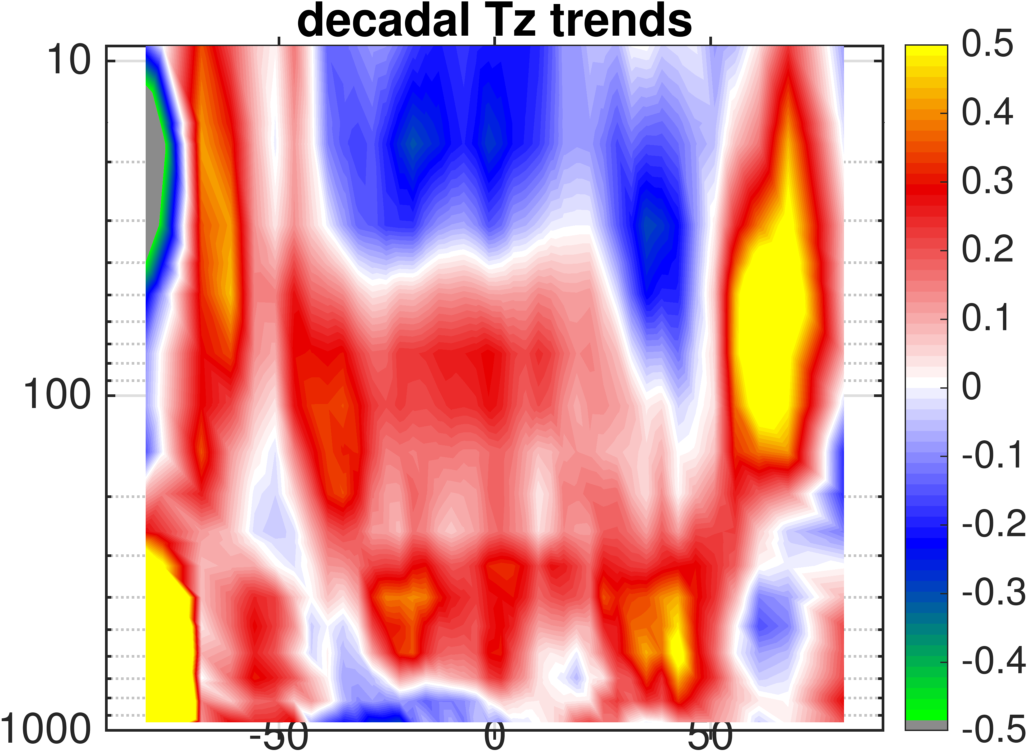
\includegraphics[width=\linewidth]{Figs/ClearAnom/umbc_clr_retr_cal_wv_rate_200209_201808.png}
\end{center}
\end{block}
\end{column}
\end{columns}

\vspace{-0.25in}

\begin{columns}
\begin{column}{0.45\columnwidth}
\begin{block}{\footnotesize $frac$ O3(z,t)}
\vspace{-0.1in}
\begin{center}
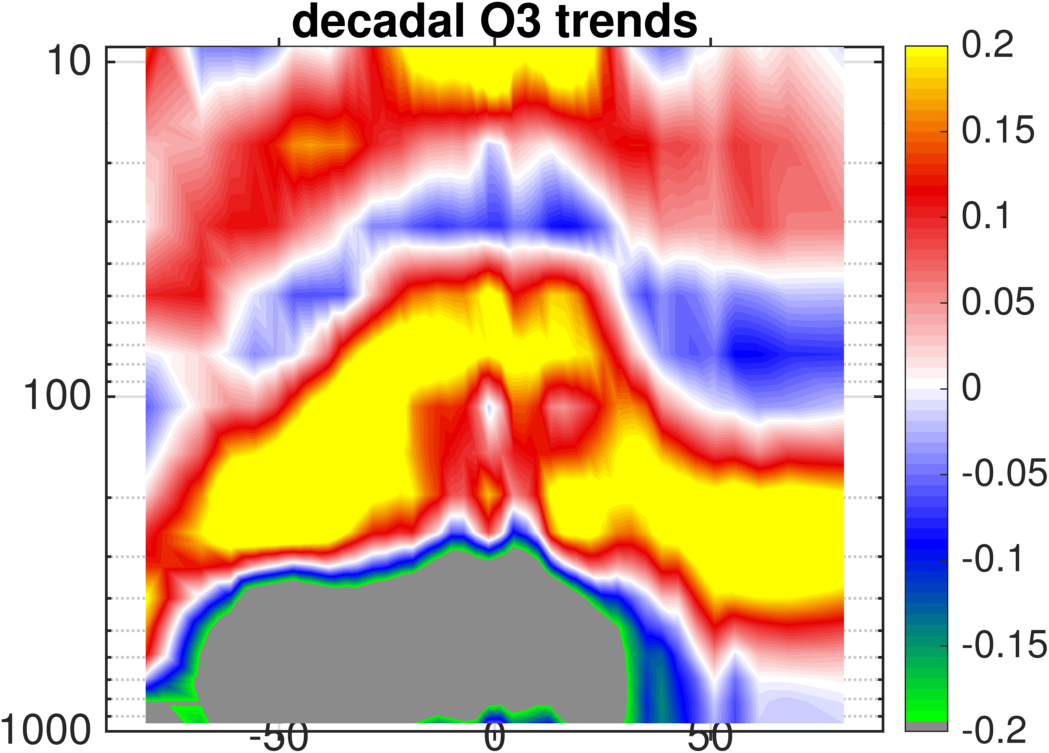
\includegraphics[width=\linewidth]{Figs/ClearAnom/umbc_clr_retr_cal_o3_rate_200209_201808.png}
\end{center}
\end{block}
\end{column}

\begin{column}{0.45\columnwidth}
%\begin{block}{\footnotesize Another Small Title}
%\vspace{-0.1in}
%\begin{center}
%\includegraphics[width=\linewidth]{{Figs/ClearAnom/umbc_clr_retr_cal_stemp_rate_200209_201808.png}
%\end{center}
%\end{block}

\end{column}
\end{columns}
\end{frame}

%%%%%%%%%%%%%%%%%%%%%%%%%%%%%%%%%%%%%%%%%%%%%%%%%%%%%%%%%%%%%%%%%%%%%%%%%%%
% ---------------------------------------------------------------------
\section{AllSky Results}

\begin{frame}
  \frametitle{AllSky Retrievals}
  \begin{itemize}
    \item \textcolor{red}{Interested in a less specialized sampling, so will now look at allsky rates}
    \item Larrabee's talk gives details (data from 2002/09 to 2018/08)
      \begin{itemize}
        \item binned into 40 equal area latitude bins (thinner in equator/thicker at polar regions)
        \item \textcolor{red}{AIRS observations randomly sampled from these bins}
        \item 16 years of data divided into 16 day averages $\rightarrow$ 365 timesteps
        \item BT anomalies and average ERA profiles for all 365 timesteps
      \end{itemize}
    \item kCARTA analytic jacobians for surface temperature, T(z), WV(z),O3(z) using TwoSlab Clouds
    \item kCARTA at t=0 to t=T to make ``finite difference'' column trace gas jacobians
          (CO2,N2O,CH4,CFC11,CFC12)
    \item SARTA for cloud jacs
    \item Using these jacobians, we retrieved T(t,z),WV(t,z),O3(t,z),[CO2(t),N2O(t),CH4(t),CFC11(t),CFC12(t),surftemp(t)]
          [cld amount/cld eff size/ cld top for liquid/ice clouds] at each of the 40 latbins $\times $ 365 timesteps
  \end{itemize}
\end{frame}

%%%%%%%%%%%%%%%%%%%%%%%%%

\section{AllSky OCEAN}
\subsection{AllSky OCEAN Rates}

\begin{frame}{Geophysical rates from spectral rates (contd)}
\vspace{-0.3in}

\begin{columns}
\begin{column}{0.55\columnwidth}
\begin{block}{\footnotesize Stemp Rates}
\vspace{-0.1in}
\begin{center}
\includegraphics[width=\linewidth]{Figs/CloudAnom/Desc_ocean/stemp_lat_rates_from_obs_specral_rates.pdf}
\end{center}
\footnotesize
This is over ocean only
\end{block}
\end{column}

\begin{column}{0.55\columnwidth}
%\begin{block}{\footnotesize Cloud param rates}
\begin{block}{\footnotesize Trace gas rates}
\vspace{-0.1in}
\begin{center}
%\includegraphics[width=\linewidth]{Figs/CloudAnom/Desc_ocean/cloudparam_lat_rates_from_obs_specral_rates.pdf}
\includegraphics[width=\linewidth]{Figs/CloudAnom/Desc_ocean/tracegas_lat_rates_from_obs_specral_rates.pdf}
\end{center}
\footnotesize
Preliminary work
\end{block}
\end{column}
\end{columns}
\end{frame}

%%%%%%%%%%

%figure(1);  aslprint_mat('/home/sergio/PAPERS/AIRS/airs_stm_sep19/allsky/Figs/CloudAnom/Desc_ocean/wv_lat_p_rates_from_obs_specral_rates',1,1,latx,playsRET,temp_ret*10);
%figure(2);  aslprint_mat('/home/sergio/PAPERS/AIRS/airs_stm_sep19/allsky/Figs/CloudAnom/Desc_ocean/tz_lat_p_rates_from_obs_specral_rates',2,1,latx,playsRET,temp_ret*10);
%figure(3);  aslprint_mat('/home/sergio/PAPERS/AIRS/airs_stm_sep19/allsky/Figs/CloudAnom/Desc_ocean/o3_lat_p_rates_from_obs_specral_rates',3,1,latx,playsRET,temp_ret*10);
%figure(7);  aslprint('/home/sergio/PAPERS/AIRS/airs_stm_sep19/allsky/Figs/CloudAnom/Desc_ocean/tracegas_lat_rates_from_obs_specral_rates.pdf');
%figure(9);  aslprint('/home/sergio/PAPERS/AIRS/airs_stm_sep19/allsky/Figs/CloudAnom/Desc_ocean/stemp_lat_rates_from_obs_specral_rates.pdf');
%figure(10); aslprint('/home/sergio/PAPERS/AIRS/airs_stm_sep19/allsky/Figs/CloudAnom/Desc_ocean/cloudparam_lat_rates_from_obs_specral_rates.pdf')

\begin{frame}{UMBC AllSky OCEAN Spectral Rates $\rightarrow$ AllSky Geophysical Rates}
%% see /home/sergio/MATLABCODE/oem_pkg_run/AIRS_new_random_scan_August2019/Plotutils/plot_all_latbins_fewlays.m
%% see /home/sergio/MATLABCODE/oem_pkg_run_sergio_AuxJacs/MakeProfs/plot_anomalies.m
\vspace{-0.35in}

\begin{columns}
\begin{column}{0.45\columnwidth}
\begin{block}{\footnotesize dT(z,t)/dt}
\vspace{-0.1in}
\begin{center}
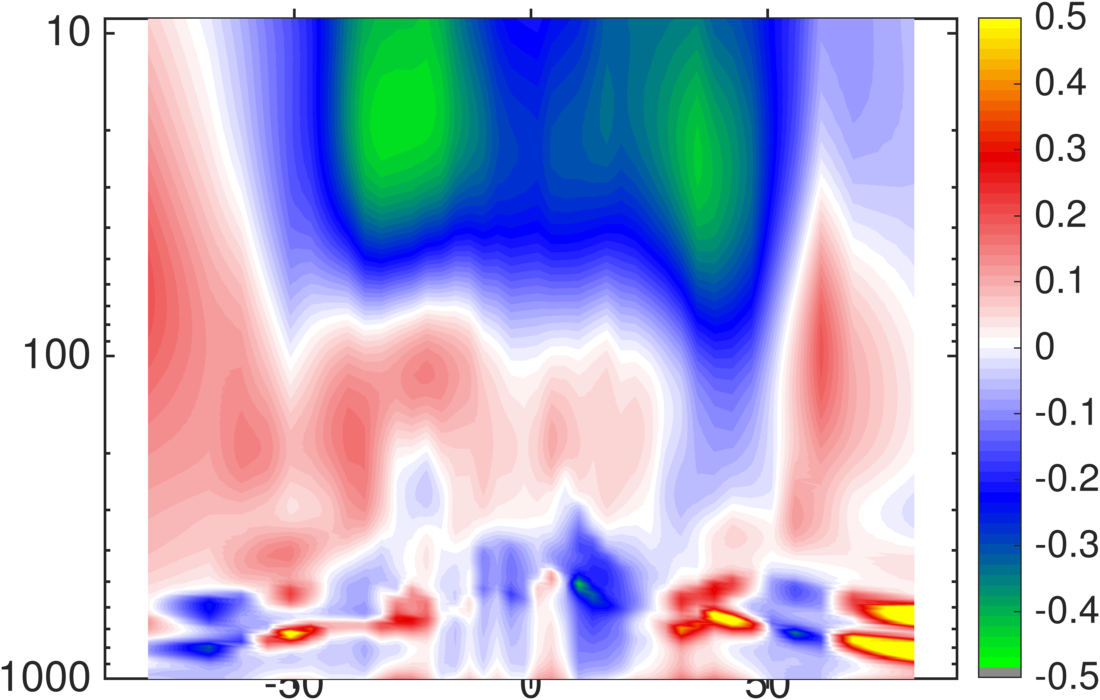
\includegraphics[width=\linewidth]{Figs/CloudAnom/Desc_ocean/tz_lat_p_rates_from_obs_specral_rates.png}
\end{center}
\end{block}
\end{column}

\begin{column}{0.45\columnwidth}
\begin{block}{\footnotesize $frac$ dWV(z,t)/dt}
\vspace{-0.1in}
\begin{center}
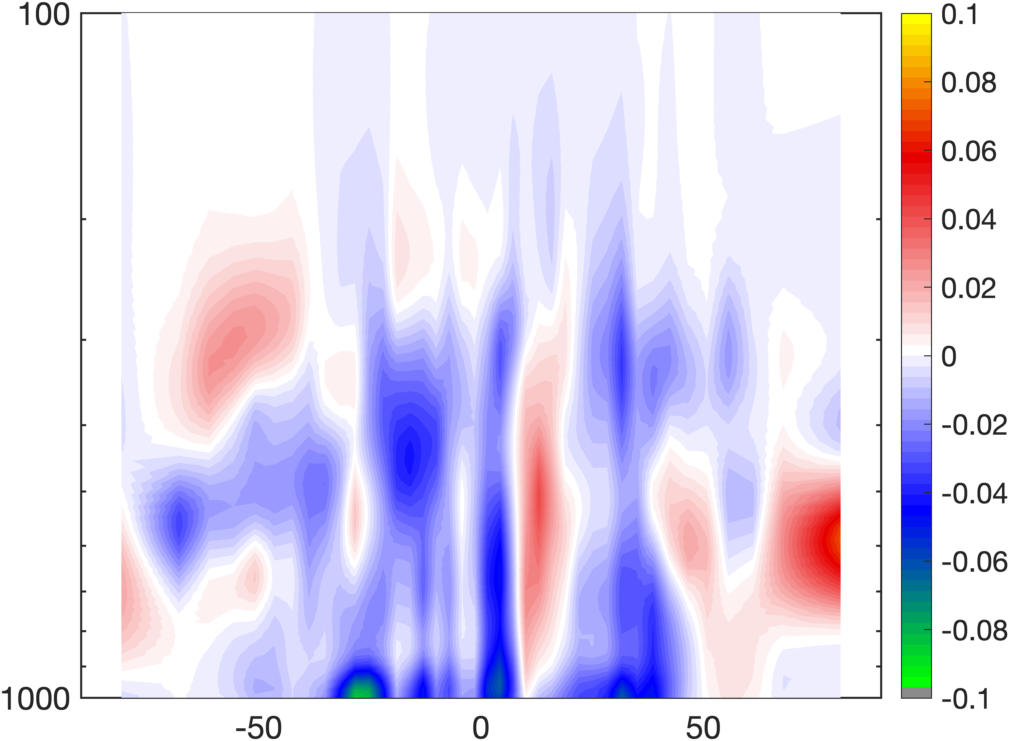
\includegraphics[width=\linewidth]{Figs/CloudAnom/Desc_ocean/wv_lat_p_rates_from_obs_specral_rates.png}
\end{center}
\end{block}
\end{column}
\end{columns}

\vspace{-0.25in}

\begin{columns}
\begin{column}{0.45\columnwidth}
\begin{block}{\footnotesize $frac$ dO3(z,t)/dt}
\vspace{-0.1in}
\begin{center}
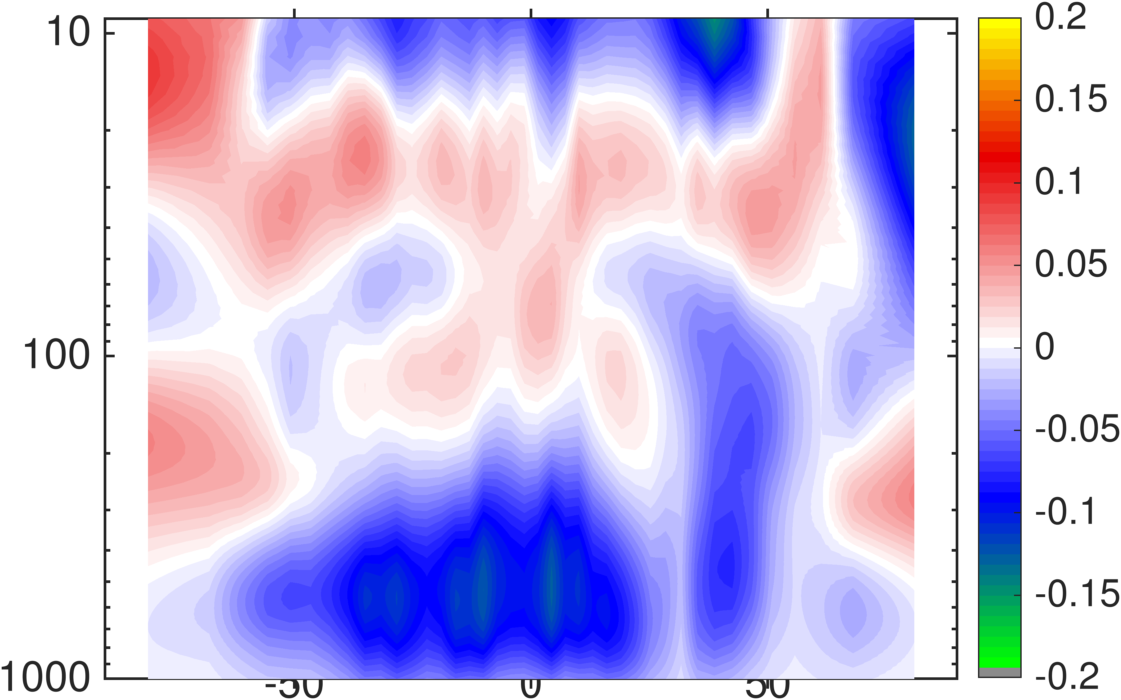
\includegraphics[width=\linewidth]{Figs/CloudAnom/Desc_ocean/o3_lat_p_rates_from_obs_specral_rates.png}
\end{center}
\end{block}
\end{column}

\begin{column}{0.45\columnwidth}
%\begin{block}{\footnotesize Another Small Title}
%\vspace{-0.1in}
%\begin{center}
%\includegraphics[width=\linewidth]{{Figs/CloudAnom/umbc_clr_retr_obs_stemp_rate_200209_201808.png}
%\end{center}
%\end{block}

\end{column}
\end{columns}
\end{frame}

%%%%%

\begin{frame}{ERA AllSky OCEAN Rates $\rightarrow$ AllSky AK $\times$ Rates}
%% see /home/sergio/MATLABCODE/oem_pkg_run/AIRS_new_random_scan_August2019/Plotutils/compute_geo_rates_ak_fewlays.m}
%% see /home/sergio/MATLABCODE/oem_pkg_run_sergio_AuxJacs/MakeProfs/plot_anomalies.m
\vspace{-0.35in}

\begin{columns}
\begin{column}{0.45\columnwidth}
\begin{block}{\footnotesize dT(z,t)/dt}
\vspace{-0.1in}
\begin{center}
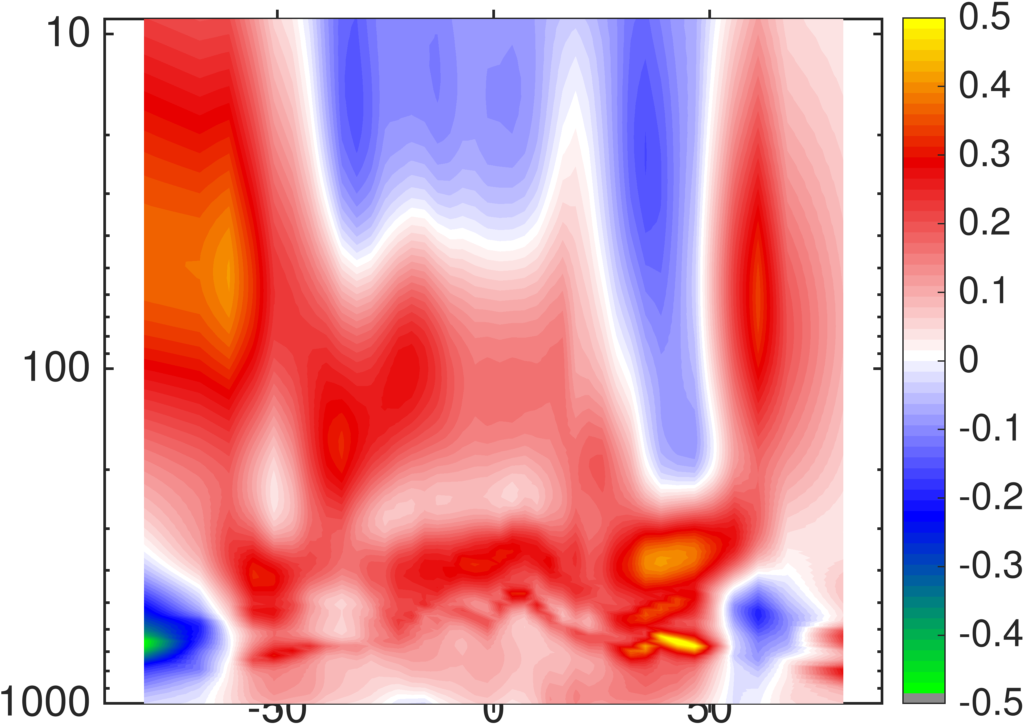
\includegraphics[width=\linewidth]{Figs/CloudAnom/Desc_ocean/ak_x_ERAtzrates.png}
\end{center}
\end{block}
\end{column}

\begin{column}{0.45\columnwidth}
\begin{block}{\footnotesize $frac$ dWV(z,t)/dt}
\vspace{-0.1in}
X\begin{center}
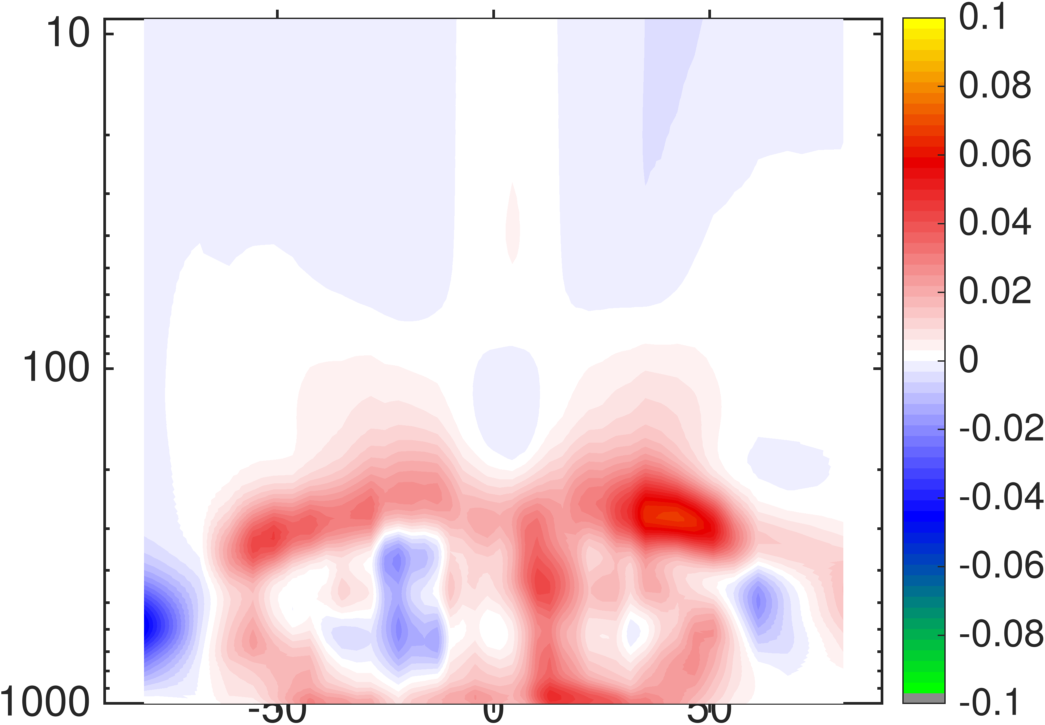
\includegraphics[width=\linewidth]{Figs/CloudAnom/Desc_ocean/ak_x_ERAwvrates.png}
\end{center}
\end{block}
\end{column}
\end{columns}

\vspace{-0.25in}

\begin{columns}
\begin{column}{0.45\columnwidth}
\begin{block}{\footnotesize $frac$ dO3(z,t)/dt}
\vspace{-0.1in}
\begin{center}
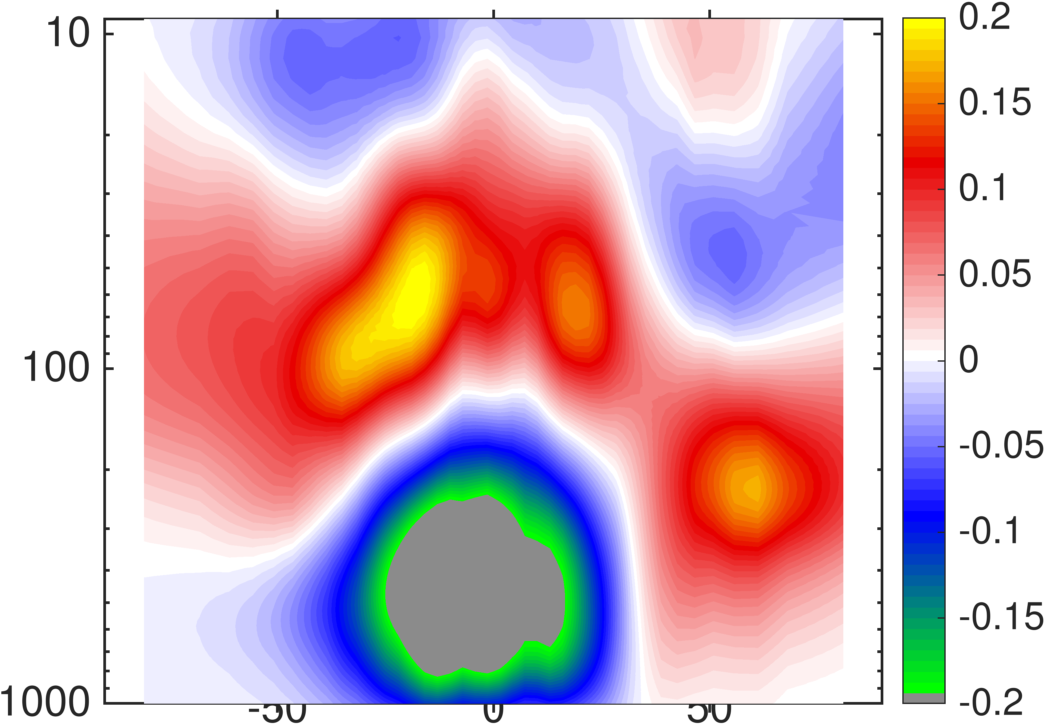
\includegraphics[width=\linewidth]{Figs/CloudAnom/Desc_ocean/ak_x_ERAo3rates.png}
\end{center}
\end{block}
\end{column}

\begin{column}{0.45\columnwidth}
%\begin{block}{\footnotesize Another Small Title}
%\vspace{-0.1in}
%\begin{center}
%\includegraphics[width=\linewidth]{{Figs/CloudAnom/umbc_clr_retr_obs_stemp_rate_200209_201808.png}
%\end{center}
%\end{block}

\end{column}
\end{columns}
\end{frame}

%%%%%

\subsection{AllSky UMBC vs ERA vs L3 Anomalies}
\begin{frame}{Tropical ERA AllSky Geophysical Anomalies}
%% see /home/sergio/MATLABCODE/oem_pkg_run_sergio_AuxJacs/MakeProfs/plot_anomalies.m
\vspace{-0.35in}

\begin{columns}
\begin{column}{0.45\columnwidth}
\begin{block}{\footnotesize T(z,t)}
\vspace{-0.1in}
\begin{center}
\includegraphics[width=\linewidth]{Figs/CloudAnom/Desc_ocean_orig/era_cld_ptemp_anom_200209_201808.png}
\end{center}
\end{block}
\end{column}

\begin{column}{0.45\columnwidth}
\begin{block}{\footnotesize $frac$ WV(z,t)}
\vspace{-0.1in}
\begin{center}
\includegraphics[width=\linewidth]{Figs/CloudAnom/Desc_ocean_orig/era_cld_wv_anom_200209_201808.png}
\end{center}
\end{block}
\end{column}
\end{columns}

\vspace{-0.25in}

\begin{columns}
\begin{column}{0.45\columnwidth}
\begin{block}{\footnotesize $frac$ O3(z,t)}
\vspace{-0.1in}
\begin{center}
\includegraphics[width=\linewidth]{Figs/CloudAnom/Desc_ocean_orig/era_cld_o3_anom_200209_201808.png}
\end{center}
\end{block}
\end{column}

\begin{column}{0.45\columnwidth}
%\begin{block}{\footnotesize Another Small Title}
%\vspace{-0.1in}
%\begin{center}
%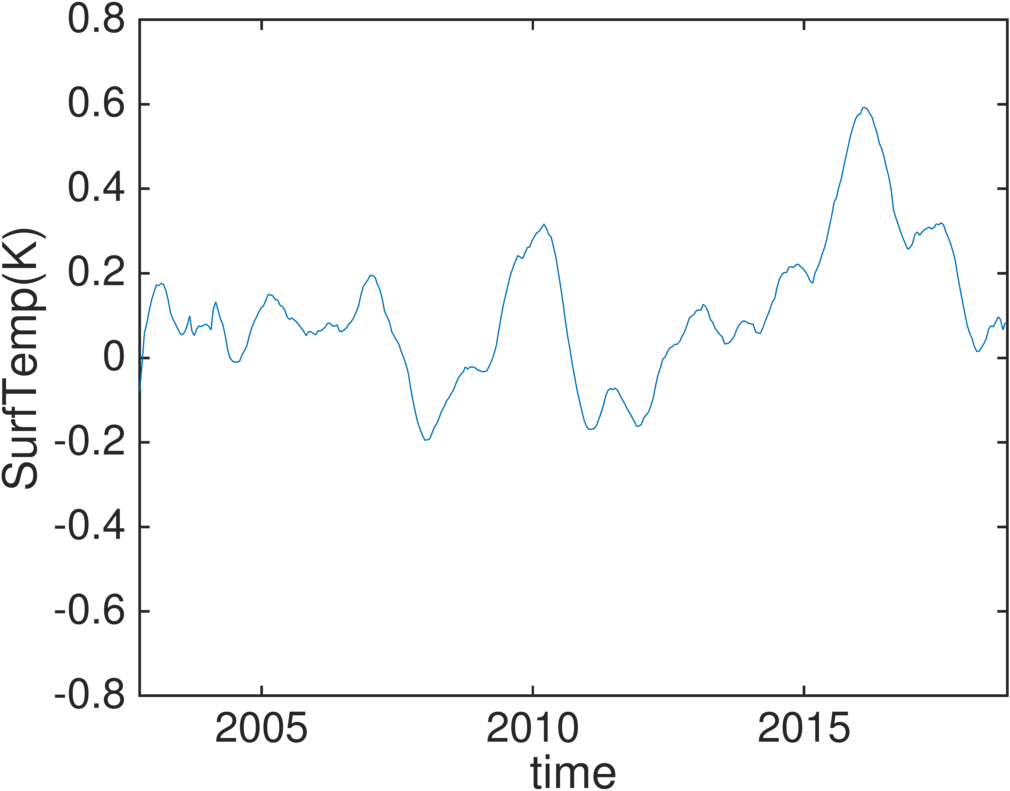
\includegraphics[width=\linewidth]{{Figs/CloudAnom/era_cld_stemp_anom_200209_201808.png}
%\end{center}
%\end{block}

\end{column}
\end{columns}
\end{frame}

%%%%%%%%%%%%%%%%%%%%%%%%%

\section{AllSky LAND/OCEAN}
\subsection{AllSky LAND/OCEAN Rates}

\begin{frame}{Geophysical rates from spectral rates (contd)}
\vspace{-0.3in}

\begin{columns}
\begin{column}{0.55\columnwidth}
\begin{block}{\footnotesize Stemp Rates}
\vspace{-0.1in}
\begin{center}
\includegraphics[width=\linewidth]{Figs/CloudAnom/Desc/stemp_lat_rates_from_obs_specral_rates.pdf}
\end{center}
\footnotesize
This is over ocean only
\end{block}
\end{column}

\begin{column}{0.55\columnwidth}
%\begin{block}{\footnotesize Cloud param rates}
\begin{block}{\footnotesize Trace gas rates}
\vspace{-0.1in}
\begin{center}
%\includegraphics[width=\linewidth]{Figs/CloudAnom/Desc/cloudparam_lat_rates_from_obs_specral_rates.pdf}
\includegraphics[width=\linewidth]{Figs/CloudAnom/Desc/tracegas_lat_rates_from_obs_specral_rates.pdf}
\end{center}
\footnotesize
Preliminary work
\end{block}
\end{column}
\end{columns}
\end{frame}

%%%%%%%%%%

%figure(1);  aslprint_mat('/home/sergio/PAPERS/AIRS/airs_stm_sep19/allsky/Figs/CloudAnom/Desc/wv_lat_p_rates_from_obs_specral_rates',1,1,latx,playsRET,temp_ret*10);
%figure(2);  aslprint_mat('/home/sergio/PAPERS/AIRS/airs_stm_sep19/allsky/Figs/CloudAnom/Desc/tz_lat_p_rates_from_obs_specral_rates',2,1,latx,playsRET,temp_ret*10);
%figure(3);  aslprint_mat('/home/sergio/PAPERS/AIRS/airs_stm_sep19/allsky/Figs/CloudAnom/Desc/o3_lat_p_rates_from_obs_specral_rates',3,1,latx,playsRET,temp_ret*10);
%figure(7);  aslprint('/home/sergio/PAPERS/AIRS/airs_stm_sep19/allsky/Figs/CloudAnom/Desc/tracegas_lat_rates_from_obs_specral_rates.pdf');
%figure(9);  aslprint('/home/sergio/PAPERS/AIRS/airs_stm_sep19/allsky/Figs/CloudAnom/Desc/stemp_lat_rates_from_obs_specral_rates.pdf');
%figure(10); aslprint('/home/sergio/PAPERS/AIRS/airs_stm_sep19/allsky/Figs/CloudAnom/Desc/cloudparam_lat_rates_from_obs_specral_rates.pdf')

\begin{frame}{UMBC AllSky OCEAN Spectral Rates $\rightarrow$ AllSky Geophysical Rates}
%% see /home/sergio/MATLABCODE/oem_pkg_run/AIRS_new_random_scan_August2019/Plotutils/plot_all_latbins_fewlays.m
%% see /home/sergio/MATLABCODE/oem_pkg_run_sergio_AuxJacs/MakeProfs/plot_anomalies.m
\vspace{-0.35in}

\begin{columns}
\begin{column}{0.45\columnwidth}
\begin{block}{\footnotesize dT(z,t)/dt}
\vspace{-0.1in}
\begin{center}
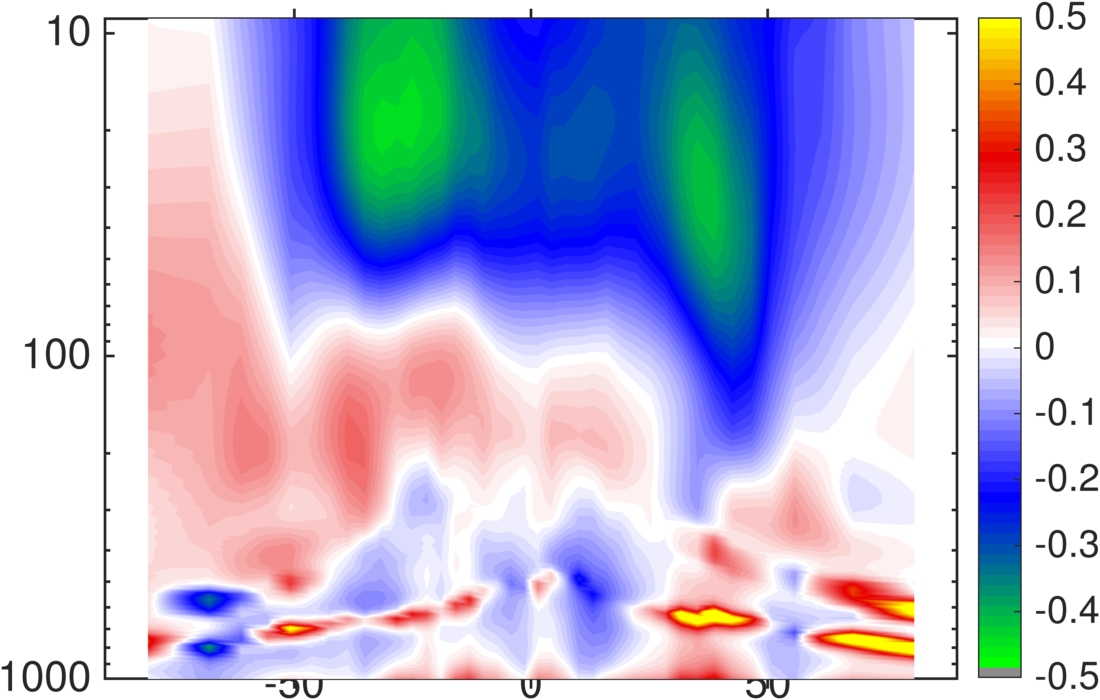
\includegraphics[width=\linewidth]{Figs/CloudAnom/Desc/tz_lat_p_rates_from_obs_specral_rates.png}
\end{center}
\end{block}
\end{column}

\begin{column}{0.45\columnwidth}
\begin{block}{\footnotesize $frac$ dWV(z,t)/dt}
\vspace{-0.1in}
\begin{center}
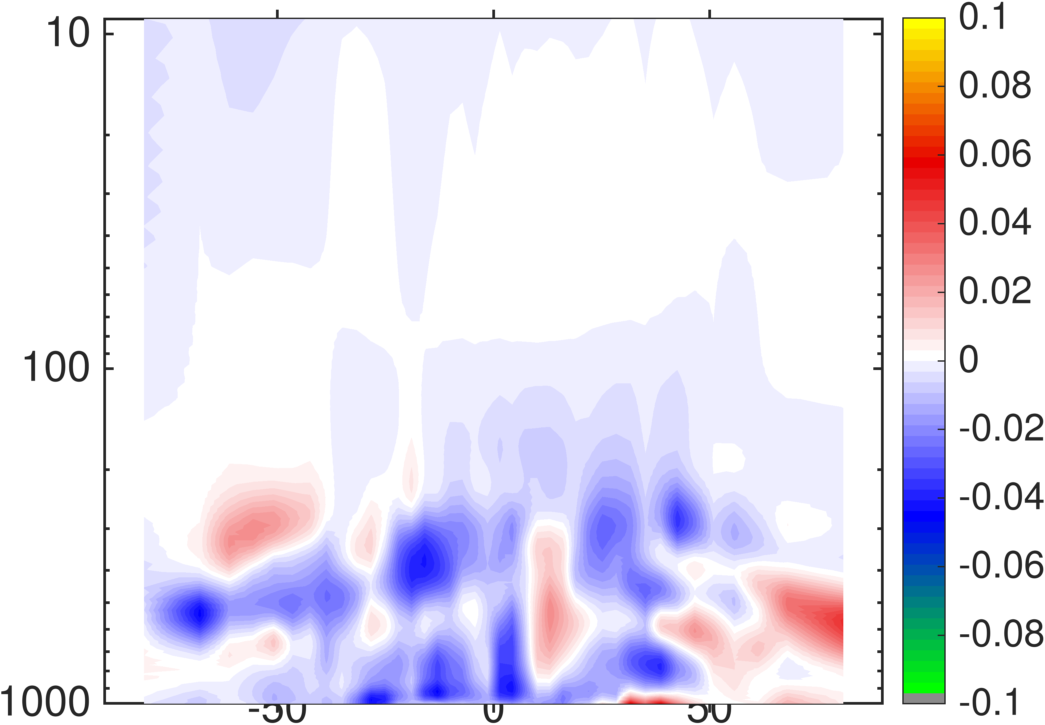
\includegraphics[width=\linewidth]{Figs/CloudAnom/Desc/wv_lat_p_rates_from_obs_specral_rates.png}
\end{center}
\end{block}
\end{column}
\end{columns}

\vspace{-0.25in}

\begin{columns}
\begin{column}{0.45\columnwidth}
\begin{block}{\footnotesize $frac$ dO3(z,t)/dt}
\vspace{-0.1in}
\begin{center}
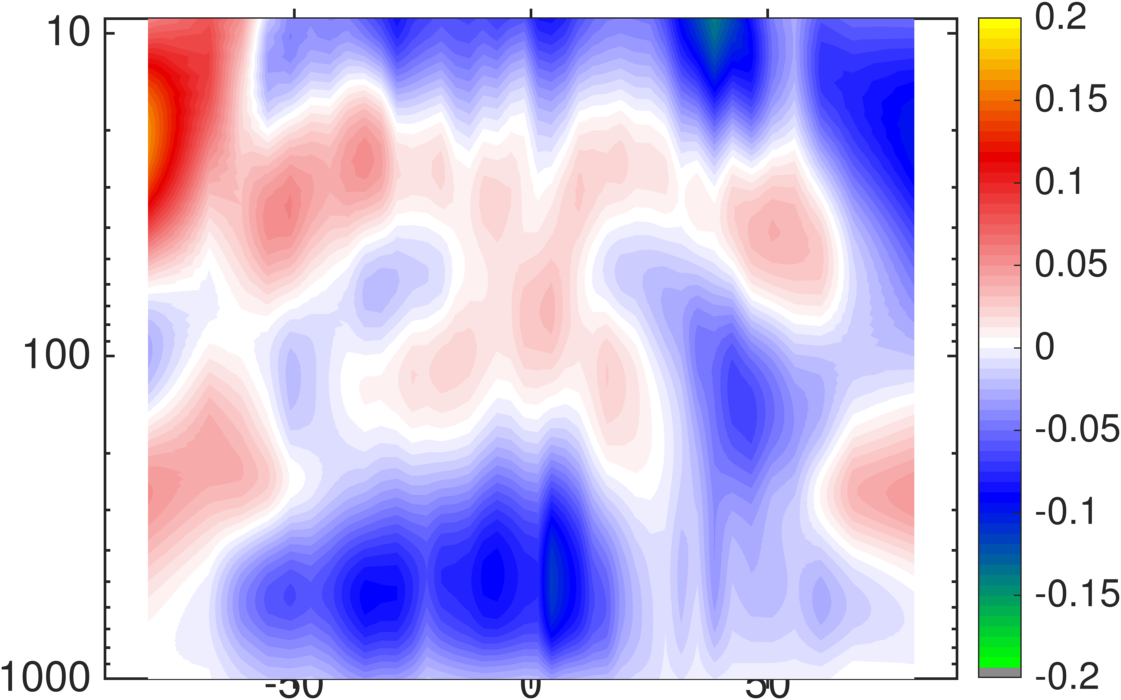
\includegraphics[width=\linewidth]{Figs/CloudAnom/Desc/o3_lat_p_rates_from_obs_specral_rates.png}
\end{center}
\end{block}
\end{column}

\begin{column}{0.45\columnwidth}
%\begin{block}{\footnotesize Another Small Title}
%\vspace{-0.1in}
%\begin{center}
%\includegraphics[width=\linewidth]{{Figs/CloudAnom/umbc_clr_retr_obs_stemp_rate_200209_201808.png}
%\end{center}
%\end{block}

\end{column}
\end{columns}
\end{frame}

%%%%%

\begin{frame}{ERA AllSky OCEAN Rates $\rightarrow$ AllSky AK $\times$ Rates}
%% see /home/sergio/MATLABCODE/oem_pkg_run/AIRS_new_random_scan_August2019/Plotutils/compute_geo_rates_ak_fewlays.m}
%% see /home/sergio/MATLABCODE/oem_pkg_run_sergio_AuxJacs/MakeProfs/plot_anomalies.m
\vspace{-0.35in}

\begin{columns}
\begin{column}{0.45\columnwidth}
\begin{block}{\footnotesize dT(z,t)/dt}
\vspace{-0.1in}
\begin{center}
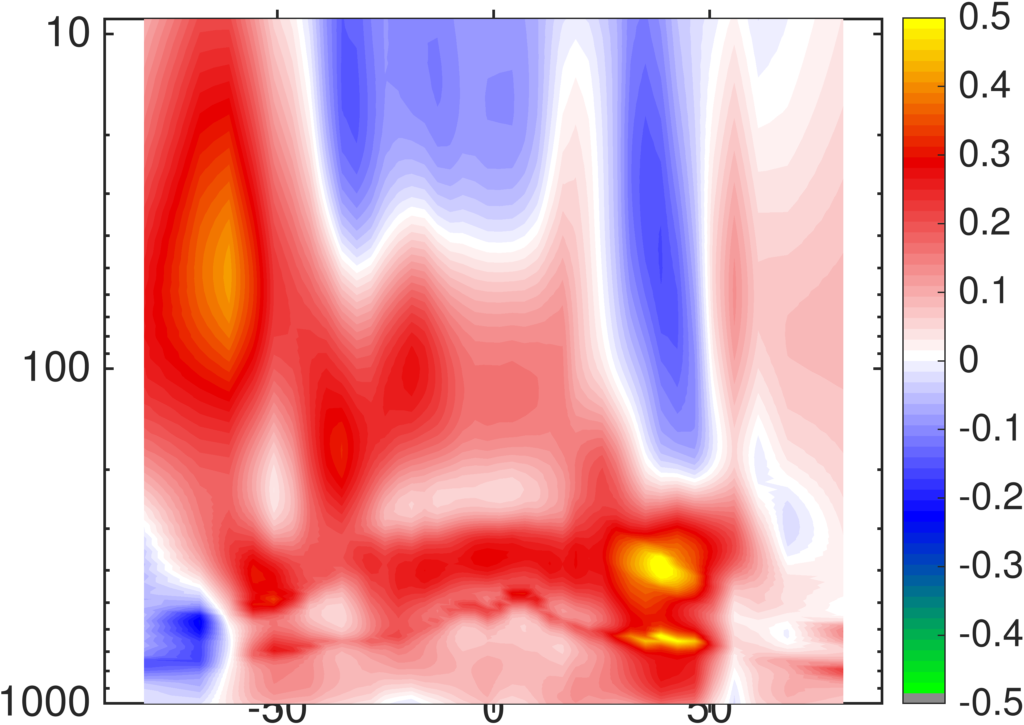
\includegraphics[width=\linewidth]{Figs/CloudAnom/Desc/ak_x_ERAtzrates.png}
\end{center}
\end{block}
\end{column}

\begin{column}{0.45\columnwidth}
\begin{block}{\footnotesize $frac$ dWV(z,t)/dt}
\vspace{-0.1in}
X\begin{center}
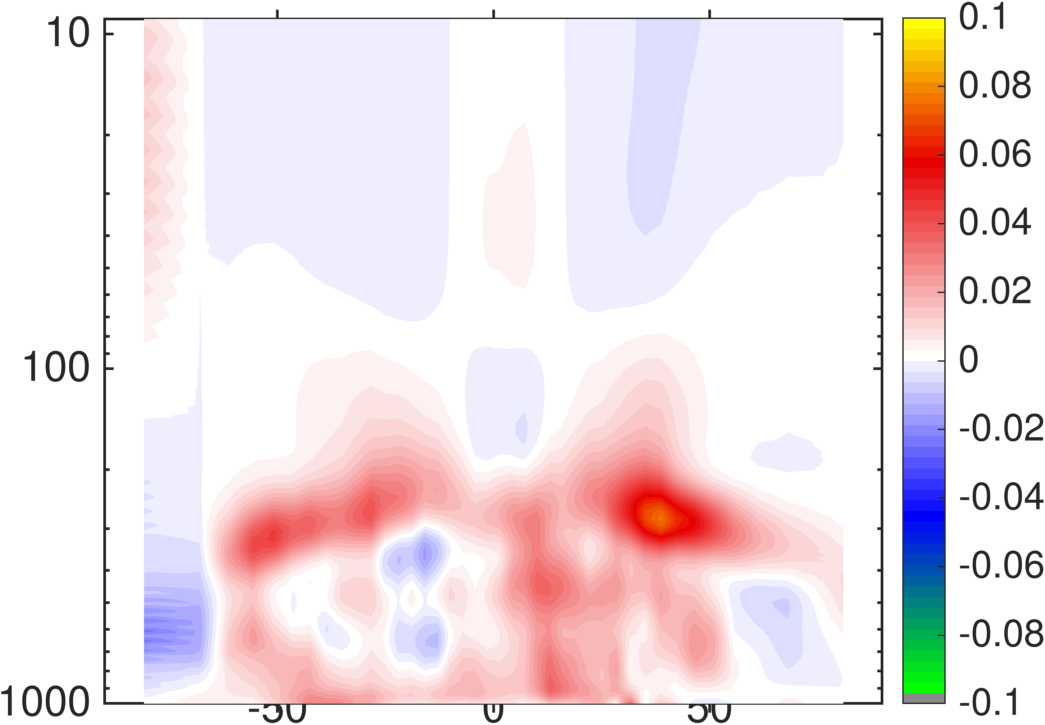
\includegraphics[width=\linewidth]{Figs/CloudAnom/Desc/ak_x_ERAwvrates.png}
\end{center}
\end{block}
\end{column}
\end{columns}

\vspace{-0.25in}

\begin{columns}
\begin{column}{0.45\columnwidth}
\begin{block}{\footnotesize $frac$ dO3(z,t)/dt}
\vspace{-0.1in}
\begin{center}
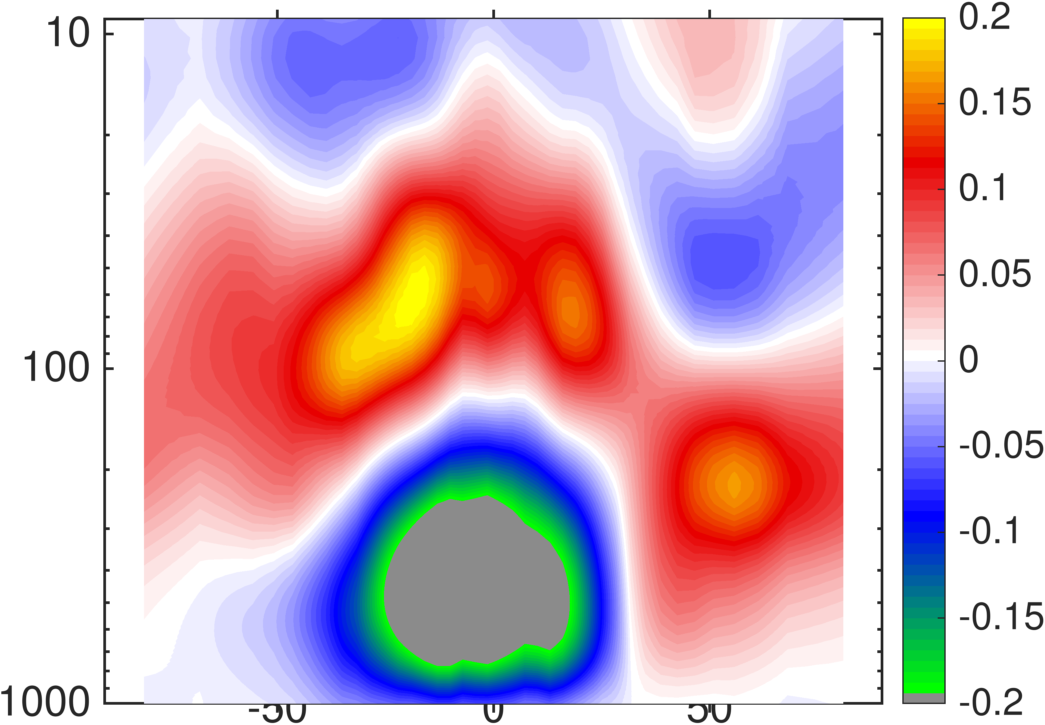
\includegraphics[width=\linewidth]{Figs/CloudAnom/Desc/ak_x_ERAo3rates.png}
\end{center}
\end{block}
\end{column}

\begin{column}{0.45\columnwidth}
%\begin{block}{\footnotesize Another Small Title}
%\vspace{-0.1in}
%\begin{center}
%\includegraphics[width=\linewidth]{{Figs/CloudAnom/umbc_clr_retr_obs_stemp_rate_200209_201808.png}
%\end{center}
%\end{block}

\end{column}
\end{columns}
\end{frame}

%%%%%

\subsection{AllSky UMBC vs ERA vs L3 Anomalies}
\begin{frame}{Tropical ERA AllSky Geophysical Anomalies}
%% see /home/sergio/MATLABCODE/oem_pkg_run_sergio_AuxJacs/MakeProfs/plot_anomalies.m
\vspace{-0.35in}

\begin{columns}
\begin{column}{0.45\columnwidth}
\begin{block}{\footnotesize T(z,t)}
\vspace{-0.1in}
\begin{center}
\includegraphics[width=\linewidth]{Figs/CloudAnom/Desc_orig/era_cld_ptemp_anom_200209_201808.png}
\end{center}
\end{block}
\end{column}

\begin{column}{0.45\columnwidth}
\begin{block}{\footnotesize $frac$ WV(z,t)}
\vspace{-0.1in}
\begin{center}
\includegraphics[width=\linewidth]{Figs/CloudAnom/Desc_orig/era_cld_wv_anom_200209_201808.png}
\end{center}
\end{block}
\end{column}
\end{columns}

\vspace{-0.25in}

\begin{columns}
\begin{column}{0.45\columnwidth}
\begin{block}{\footnotesize $frac$ O3(z,t)}
\vspace{-0.1in}
\begin{center}
\includegraphics[width=\linewidth]{Figs/CloudAnom/Desc_orig/era_cld_o3_anom_200209_201808.png}
\end{center}
\end{block}
\end{column}

\begin{column}{0.45\columnwidth}
%\begin{block}{\footnotesize Another Small Title}
%\vspace{-0.1in}
%\begin{center}
%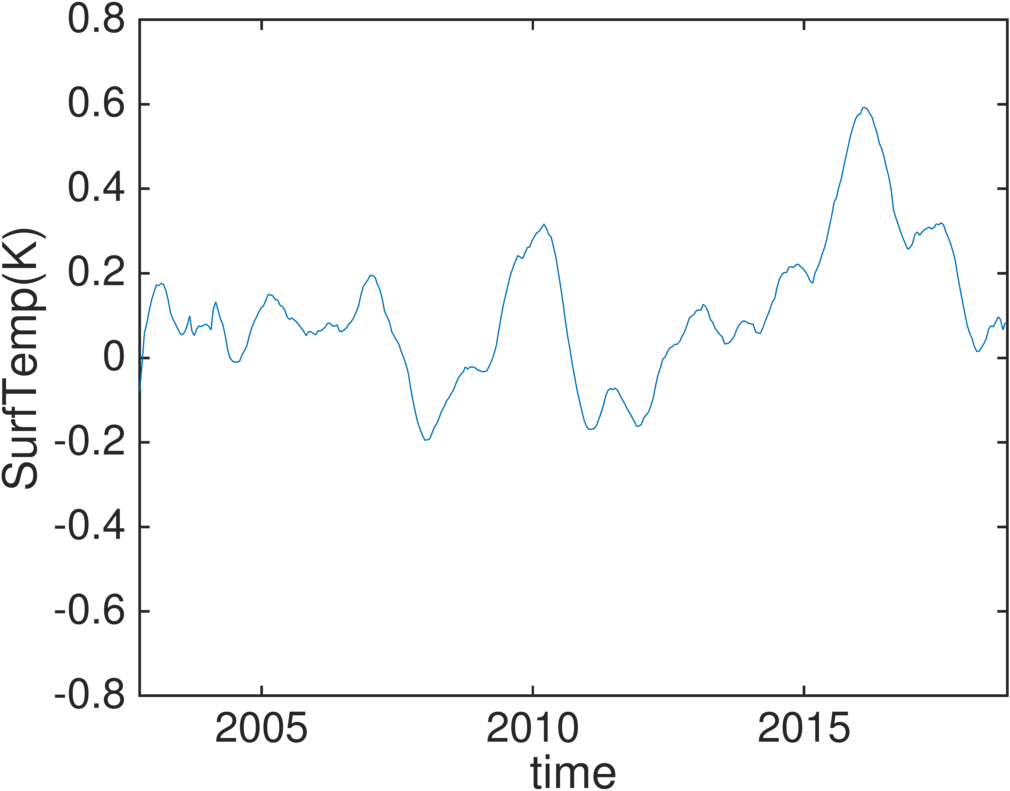
\includegraphics[width=\linewidth]{{Figs/CloudAnom/era_cld_stemp_anom_200209_201808.png}
%\end{center}
%\end{block}

\end{column}
\end{columns}
\end{frame}

%%%%%

\end{document}

